%  LaTeX support: latex@mdpi.com 
%  For support, please attach all files needed for compiling as well as the log file, and specify your operating system, LaTeX version, and LaTeX editor.

%=================================================================
\documentclass[remotesensing,article,accept,pdftex,moreauthors]{Definitions/mdpi} 
% \documentclass[journal,article,submit,pdftex,moreauthors]{Definitions/mdpi} 

%--------------------
% Class Options:
%--------------------
%----------
% journal
%----------
% Choose between the following MDPI journals:
% acoustics, actuators, addictions, admsci, adolescents, aerobiology, aerospace, agriculture, agriengineering, agrochemicals, agronomy, ai, air, algorithms, allergies, alloys, analytica, analytics, anatomia, animals, antibiotics, antibodies, antioxidants, applbiosci, appliedchem, appliedmath, applmech, applmicrobiol, applnano, applsci, aquacj, architecture, arm, arthropoda, arts, asc, asi, astronomy, atmosphere, atoms, audiolres, automation, axioms, bacteria, batteries, bdcc, behavsci, beverages, biochem, bioengineering, biologics, biology, biomass, biomechanics, biomed, biomedicines, biomedinformatics, biomimetics, biomolecules, biophysica, biosensors, biotech, birds, bloods, blsf, brainsci, breath, buildings, businesses, cancers, carbon, cardiogenetics, catalysts, cells, ceramics, challenges, chemengineering, chemistry, chemosensors, chemproc, children, chips, cimb, civileng, cleantechnol, climate, clinpract, clockssleep, cmd, coasts, coatings, colloids, colorants, commodities, compounds, computation, computers, condensedmatter, conservation, constrmater, cosmetics, covid, crops, cryptography, crystals, csmf, ctn, curroncol, cyber, dairy, data, ddc, dentistry, dermato, dermatopathology, designs, devices, diabetology, diagnostics, dietetics, digital, disabilities, diseases, diversity, dna, drones, dynamics, earth, ebj, ecologies, econometrics, economies, education, ejihpe, electricity, electrochem, electronicmat, electronics, encyclopedia, endocrines, energies, eng, engproc, entomology, entropy, environments, environsciproc, epidemiologia, epigenomes, est, fermentation, fibers, fintech, fire, fishes, fluids, foods, forecasting, forensicsci, forests, foundations, fractalfract, fuels, future, futureinternet, futurepharmacol, futurephys, futuretransp, galaxies, games, gases, gastroent, gastrointestdisord, gels, genealogy, genes, geographies, geohazards, geomatics, geosciences, geotechnics, geriatrics, grasses, gucdd, hazardousmatters, healthcare, hearts, hemato, hematolrep, heritage, higheredu, highthroughput, histories, horticulturae, hospitals, humanities, humans, hydrobiology, hydrogen, hydrology, hygiene, idr, ijerph, ijfs, ijgi, ijms, ijns, ijpb, ijtm, ijtpp, ime, immuno, informatics, information, infrastructures, inorganics, insects, instruments, inventions, iot, j, jal, jcdd, jcm, jcp, jcs, jcto, jdb, jeta, jfb, jfmk, jimaging, jintelligence, jlpea, jmmp, jmp, jmse, jne, jnt, jof, joitmc, jor, journalmedia, jox, jpm, jrfm, jsan, jtaer, jvd, jzbg, kidneydial, kinasesphosphatases, knowledge, land, languages, laws, life, liquids, literature, livers, logics, logistics, lubricants, lymphatics, machines, macromol, magnetism, magnetochemistry, make, marinedrugs, materials, materproc, mathematics, mca, measurements, medicina, medicines, medsci, membranes, merits, metabolites, metals, meteorology, methane, metrology, micro, microarrays, microbiolres, micromachines, microorganisms, microplastics, minerals, mining, modelling, molbank, molecules, mps, msf, mti, muscles, nanoenergyadv, nanomanufacturing,\gdef\@continuouspages{yes}} nanomaterials, ncrna, ndt, network, neuroglia, neurolint, neurosci, nitrogen, notspecified, %%nri, nursrep, nutraceuticals, nutrients, obesities, oceans, ohbm, onco, %oncopathology, optics, oral, organics, organoids, osteology, oxygen, parasites, parasitologia, particles, pathogens, pathophysiology, pediatrrep, pharmaceuticals, pharmaceutics, pharmacoepidemiology,\gdef\@ISSN{2813-0618}\gdef\@continuous pharmacy, philosophies, photochem, photonics, phycology, physchem, physics, physiologia, plants, plasma, platforms, pollutants, polymers, polysaccharides, poultry, powders, preprints, proceedings, processes, prosthesis, proteomes, psf, psych, psychiatryint, psychoactives, publications, quantumrep, quaternary, qubs, radiation, reactions, receptors, recycling, regeneration, religions, remotesensing, reports, reprodmed, resources, rheumato, risks, robotics, ruminants, safety, sci, scipharm, sclerosis, seeds, sensors, separations, sexes, signals, sinusitis, skins, smartcities, sna, societies, socsci, software, soilsystems, solar, solids, spectroscj, sports, standards, stats, std, stresses, surfaces, surgeries, suschem, sustainability, symmetry, synbio, systems, targets, taxonomy, technologies, telecom, test, textiles, thalassrep, thermo, tomography, tourismhosp, toxics, toxins, transplantology, transportation, traumacare, traumas, tropicalmed, universe, urbansci, uro, vaccines, vehicles, venereology, vetsci, vibration, virtualworlds, viruses, vision, waste, water, wem, wevj, wind, women, world, youth, zoonoticdis 
% For posting an early version of this manuscript as a preprint, you may use "preprints" as the journal. Changing "submit" to "accept" before posting will remove line numbers.

%---------
% article
%---------
% The default type of manuscript is "article", but can be replaced by: 
% abstract, addendum, article, book, bookreview, briefreport, casereport, comment, commentary, communication, conferenceproceedings, correction, conferencereport, entry, expressionofconcern, extendedabstract, datadescriptor, editorial, essay, erratum, hypothesis, interestingimage, obituary, opinion, projectreport, reply, retraction, review, perspective, protocol, shortnote, studyprotocol, systematicreview, supfile, technicalnote, viewpoint, guidelines, registeredreport, tutorial
% supfile = supplementary materials

%----------
% submit
%----------
% The class option "submit" will be changed to "accept" by the Editorial Office when the paper is accepted. This will only make changes to the frontpage (e.g., the logo of the journal will get visible), the headings, and the copyright information. Also, line numbering will be removed. Journal info and pagination for accepted papers will also be assigned by the Editorial Office.

%------------------
% moreauthors
%------------------
% If there is only one author the class option oneauthor should be used. Otherwise use the class option moreauthors.

%---------
% pdftex
%---------
% The option pdftex is for use with pdfLaTeX. Remove "pdftex" for (1) compiling with LaTeX & dvi2pdf (if eps figures are used) or for (2) compiling with XeLaTeX.

%=================================================================
% MDPI internal commands - do not modify
\firstpage{1} 
\makeatletter 
\setcounter{page}{\@firstpage} 
\makeatother
\pubvolume{15}
\issuenum{1}
\articlenumber{0}
\pubyear{2023}
\copyrightyear{2023}
\externaleditor{Academic Editor: {Yanjun Su} %MDPI: Please add this part. no problem -W
}
\datereceived{11 May 2023} 
\daterevised{6 June 2023} % Comment out if no revised date
\dateaccepted{20 June 2023} 
\datepublished{ } 
%\datecorrected{} % For corrected papers: "Corrected: XXX" date in the original paper.
%\dateretracted{} % For corrected papers: "Retracted: XXX" date in the original paper.
\hreflink{https://doi.org/} % If needed use \linebreak
%\doinum{}
%\pdfoutput=1 % Uncommented for upload to arXiv.org

%=================================================================
% Add packages and commands here. The following packages are loaded in our class file: fontenc, inputenc, calc, indentfirst, fancyhdr, graphicx, epstopdf, lastpage, ifthen, float, amsmath, amssymb, lineno, setspace, enumitem, mathpazo, booktabs, titlesec, etoolbox, tabto, xcolor, colortbl, soul, multirow, microtype, tikz, totcount, changepage, attrib, upgreek, array, tabularx, pbox, ragged2e, tocloft, marginnote, marginfix, enotez, amsthm, natbib, hyperref, cleveref, scrextend, url, geometry, newfloat, caption, draftwatermark, seqsplit
% cleveref: load \crefname definitions after \begin{document}

%=================================================================
% Please use the following mathematics environments: Theorem, Lemma, Corollary, Proposition, Characterization, Property, Problem, Example, ExamplesandDefinitions, Hypothesis, Remark, Definition, Notation, Assumption
%% For proofs, please use the proof environment (the amsthm package is loaded by the MDPI class).

%=================================================================

\Title{Identification of Abandoned Logging Roads in Point Reyes National Seashore}
%MDPI: IMPORTANT INFORMATION: 
%1. Please ensure that this is the final version that can be published and confirm that you will require no further changes from hereon. !agreed -W
%2. Please proof on this version as we have already done the English editing and formatting changes. Please do the proofreading with track changes. Do reply all comments and do not delete them. Thank you !agreed -W
%3. Please provide GA. Graphical abstract is recommended for every manuscript to help readers to comprehend (The detailed requirements for the GA are listed in the email “Please Provide Graphical Abstract”, please pay attention)




\TitleCitation{Identification of Abandoned Logging Roads in Point Reyes National Seashore}

% Author Orchid ID: enter ID or remove command
\newcommand{\orcidauthorA}{0000-0003-1158-3830} % Add \orcidA{} behind the author's name
%\newcommand{\orcidauthorB}{XXX} % Add \orcidB{} behind the author's name
\newcommand{\orcidauthorC}{0000-0001-7805-6272}



\Author{William Wiskes *\orcidA{}, %MDPI: 1. Please carefully check the accuracy of ALL names and affiliations.
%2. The name of this author is different from the one submitted online at susy.mdpi.com (William Wiskes). Please confirm which one is correct. !Either is fine with me, However since you were expecting William Wiskes, I will just use that name -W
 Leonhard Blesius and Ellen Hines \orcidC{}}



\AuthorNames{William Wiskes, Leonhard Blesius and Ellen Hines}


\AuthorCitation{Wiskes, %MDPI: Please carefully check the accuracy of names and affiliations. !I have now changed -W
 W.; Blesius, L.; Hines, E.}



\address[1]{%
Department of Geography and Environment, San Francisco State University, 1600 Holloway Avenue, %MDPI: We switched the address order, please confirm. This is fine -W
 San~Francisco,~CA~94132,~USA; william.wiskes@usda.gov (W.W.); lblesius@sfsu.edu (L.B.)
 
 Estuary \& Ocean Sciences Center, San Francisco State University, Tiburon, CA, USA; ehines@sfsu.edu (E.H.)}


% Contact information of the corresponding author
\corres{\hangafter=1 \hangindent=1.05em \hspace{-0.82em} Correspondence: william.wiskes@usda.gov}


% Current address and/or shared authorship
% \firstnote{Current address: Affiliation 3.} 
% \secondnote{These authors contributed equally to this work.}
% The commands \thirdnote{} till \eighthnote{} are available for further notes

%\simplesumm{} % Simple summary

%\conference{} % An extended version of a conference paper

% Abstract (Do not insert blank lines, i.e. \\) 
\abstract{Temporary roads are often placed in mountainous regions for logging purposes but then never decommissioned and removed. These abandoned forest roads often have unwanted environmental consequences. They can lead to altered hydrological regimes, excess erosion, and mass wasting events. These events can affect sediment budgets in streams, with negative consequences for anadromous fish populations. Maps of these roads are frequently non-existent; therefore, methods need to be created to identify and locate these roads for decommissioning. Abandoned logging roads in the Point Reyes National Seashore in California, an area partially under heavy forest canopy, were mapped using object-based image processing in concert with machine learning. High-resolution Q1 LiDAR point clouds from 2019 were used to create a bare earth model of the region, from which a slope model was derived. This slope model was then subjected to segmentation algorithms to identify and isolate regions of differing slopes. Regions of differing slopes were then used in a convolutional neural network (CNN), and a maximum likelihood classifier was used to delineate the historic road network. %Please check intended meaning has been retained. !Yes this looks good -W
The accuracy assessment was conducted using historic aerial photos of the state of the region post-logging, along with ground surveys to verify the presence of logging roads in areas of question. This method was successfully able to identify road networks with a precision of 0.991 and an accuracy of 0.992. It was also found that the CNN was able to identify areas of highest disturbance to the slope gradient. This methodology is a valuable tool for decision makers who need to identify areas of high disturbance in order to mitigate adverse effects.}

% Keywords
\keyword{LiDAR; object-based image analysis; image segmentation; CNN; machine learning; maximum likelihood classifier; feature extraction; aerial photos; forest roads; logging roads} 

% The fields PACS, MSC, and JEL may be left empty or commented out if not applicable
%\PACS{J0101}
%\MSC{}
%\JEL{}

%%%%%%%%%%%%%%%%%%%%%%%%%%%%%%%%%%%%%%%%%%
% Only for the journal Diversity
%\LSID{\url{http://}}

%%%%%%%%%%%%%%%%%%%%%%%%%%%%%%%%%%%%%%%%%%
% Only for the journal Applied Sciences
%\featuredapplication{Authors are encouraged to provide a concise description of the specific application or a potential application of the work. This section is not mandatory.}
%%%%%%%%%%%%%%%%%%%%%%%%%%%%%%%%%%%%%%%%%%

%%%%%%%%%%%%%%%%%%%%%%%%%%%%%%%%%%%%%%%%%%
% Only for the journal Data
%\dataset{DOI number or link to the deposited data set if the data set is published separately. If the data set shall be published as a supplement to this paper, this field will be filled by the journal editors. In this case, please submit the data set as a supplement.}
%\datasetlicense{License under which the data set is made available (CC0, CC-BY, CC-BY-SA, CC-BY-NC, etc.)}

%%%%%%%%%%%%%%%%%%%%%%%%%%%%%%%%%%%%%%%%%%
% Only for the journal Toxins
%\keycontribution{The breakthroughs or highlights of the manuscript. Authors can write one or two sentences to describe the most important part of the paper.}

%%%%%%%%%%%%%%%%%%%%%%%%%%%%%%%%%%%%%%%%%%
% Only for the journal Encyclopedia
%\encyclopediadef{For entry manuscripts only: please provide a brief overview of the entry title instead of an abstract.}

%%%%%%%%%%%%%%%%%%%%%%%%%%%%%%%%%%%%%%%%%%
% Only for the journal Advances in Respiratory Medicine
%\addhighlights{yes}
%\renewcommand{\addhighlights}{%

%\noindent This is an obligatory section in “Advances in Respiratory Medicine”, whose goal is to increase the discoverability and readability of the article via search engines and other scholars. Highlights should not be a copy of the abstract, but a simple text allowing the reader to quickly and simplified find out what the article is about and what can be cited from it. Each of these parts should be devoted up to 2~bullet points.\vspace{3pt}\\
%\textbf{What are the main findings?}
% \begin{itemize}[labelsep=2.5mm,topsep=-3pt]
% \item First bullet.
% \item Second bullet.
% \end{itemize}\vspace{3pt}
%\textbf{What is the implication of the main finding?}
% \begin{itemize}[labelsep=2.5mm,topsep=-3pt]
% \item First bullet.
% \item Second bullet.
% \end{itemize}
%}
%\usepackage{rotating}%sidewaystable
%%%%%%%%%%%%%%%%%%%%%%%%%%%%%%%%%%%%%%%%%%
\begin{document}

%%%%%%%%%%%%%%%%%%%%%%%%%%%%%%%%%%%%%%%%%%
% \setcounter{section}{-1} %% Remove this when starting to work on the template.
% \section{How to Use this Template}

% The template details the sections that can be used in a manuscript. Note that the order and names of article sections may differ from the requirements of the journal (e.g., the positioning of the Materials and Methods section). Please check the instructions on the authors' page of the journal to verify the correct order and names. For any questions, please contact the editorial office of the journal or support@mdpi.com. For LaTeX-related questions please contact latex@mdpi.com.%\endnote{This is an endnote.} % To use endnotes, please un-comment \printendnotes below (before References). Only journal Laws uses \footnote.

% % The order of the section titles is different for some journals. Please refer to the "Instructions for Authors” on the journal homepage.

\section{Introduction}

Roads are often placed in wild, forested regions for a variety of reasons. Whether constructed for recreation, infrastructure, fire combat, or logging, these roads are often poorly documented, and their precise location may become lost due to infrequent use, changes in the morphology of the area, and vegetation encroachment \cite{becker, sherba}. This results in networks of roads, many of which have become neglected, fragmented, and difficult to find for remediation purposes. Having maps of these historic lost roads is essential for decommissioning efforts \cite{white}.

Abandoned forest roads, specifically abandoned logging roads, typically are composed of compacted soil \cite{rab}. This compacted soil can act as a semi-impervious surface and divert water flow from one watershed to another \cite{troendle}. Watersheds in forested regions are especially susceptible to mass wasting events and enhanced sediment flows in areas where the natural geomorphological processes have been disturbed \cite{luce}. Logging roads in forested regions can bring subsurface flow to the surface and accelerate erosion with overland flow \cite{underwood}, which can result in incisions into the natural landscape slope gradient. These incisions can provide a direct path for concentrated overland flow containing increased sediment loads to stream channels \cite{douglas}. This accelerated erosion can deposit fine sediment into the drainage basin and negatively affect fish habitat in streams. In summary, roads can limit infiltration, cause surface runoff, increase the rate of fine sediment production, and trigger mass wasting events \cite{wemple}. Increased sediment loads in watersheds have been shown to affect the ecological composition of many forest species \cite{wong}. 

In the Point Reyes National Seashore, 154 different fish species are known to utilize the aquatic habitat \cite{kelly}. Two of these have been listed as species of special concern: the coho salmon ({\it Oncorhynchus kissutch}), and the steelhead trout ({\it Oncorhynchus mykiss irideus}) \cite{ketcham}. These are anadromous fish who depend entirely on gravely freshwater stream beds for habitat and breeding success \cite{gronsdahl}. Logging roads are known to affect the spawning rates and habitat suitability in anadromous fish populations \cite{jacob}, primarily because logging roads increase fine sediment loads to stream channels and decrease the amount of available gravel \cite{baxter}. Increased sediment flow into stream beds from logging roads can persist up to 80 years past the logging event \cite{moore}, showing the need to identify these roads despite their age. Decommissioning roads has been found to return sediment loads to their natural levels \cite{ahnert, douglas}. Identifying and removing sources of high sediment loads should be a priority for any habitat remediation project for these sensitive species \cite{gronsdahl, jacob}.  

Much research has been undertaken to identify roads from both imagery and light detection and ranging (LiDAR) point clouds \cite{li, yong, lillesand, mena, wang, white, yucong}, but limited work has been undertaken to identify logging roads under vegetation \cite{sherba}. Dense vegetation obscures the chance of road identification from aerial or satellite imagery \cite{wang}, whereas LiDAR has the ability to penetrate through canopy and gather an accurate 3d interpretation of the ground underneath \cite{stoker}. However, because logging roads are often dirt or gravel, their uniform features, such as their curb height~\cite{li} or intensity \cite{yong}, which would traditionally be used in processes meant for extracting road forms from LiDAR, cannot be used. Additionally, logging road networks often become highly fragmented over time, making the extraction of complete road networks more~difficult. 

Object-based image analysis (OBIA) is the process of clustering pixels into regions that correspond to “individual surfaces, objects, or natural parts of objects” (\cite{preetha}, p.~576). This contrasts with the more traditional pixel-based methods where the spectral signature of the pixel alone is the primarily consideration, typically neglecting spatial aspects such as the size and shape of the area being classified, or topological relationships \cite{khatami}. This often results in `salt and pepper' classifications, where classes overlap, mix, and cause errors \cite{lu}. OBIA has been shown to perform with higher accuracy, primarily because, in addition to spectral values, OBIA can also focus on an object's shape relative to the scene as well as the object's texture and proximity to other objects \cite{karami}.

Convolutional neural networks (CNN) are a machine learning method that has shown great promise in remote sensing in recent years, especially in conjunction with object-based image analysis \cite{ferreira}. CNNs have been used to improve image classifications through their ability to automatically extract spatial patterns of images using a set of convolution and pooling operations to learn specific objects’ characteristics \cite{zhang}. This can be an especially accurate tool when combined with OBIA \cite{martins}. OBIA’s ability to preserve objects and edges, when integrated with CNNs, can be used to generate robust, consistent, and fully automated classifications \cite{robson}.

When acquiring LiDAR for road detection purposes, high point density is required in heavily forested regions. While some studies have experimented with using LiDAR files with as few as 6 pulses/m$^2$ \cite{white}, it should be noted that the roads in question were not abandoned or in dense forests; therefore, detecting them was less of a problem. Maintained roads reflect back more LiDAR points because of a lack of ground and canopy vegetation, and they tend to not be fragmented, which makes the detection and extraction process more straightforward \cite{li}. In addition, many studies have used intensity images derived from LiDAR to detect roads, although intensity has proven to be less useful for road detection when the roads are unpaved \cite{yong, white}.  

Forested roads have more vegetation through which the LiDAR must penetrate to get an accurate ground return. Thus, unmaintained roads need considerably higher point density to be detected. Because of this, it is recommended to have ideally more than 6~pulses/m$^2$ for densely vegetated regions \cite{sherba}. 

It is the goal of this project to develop a set of segmentation and classification criteria to map abandoned, overgrown logging roads in Point Reyes National Seashore, California using LiDAR point cloud tiles, OBIA, and CNN. 

These efforts in identifying abandoned logging roads will help add to the body of knowledge at the disposal of environmental planners aiming to remediate damaged habitat. Managers at Point Reyes National Seashore have identified this specific issue to be the top   priority on their list of management needs \cite{becker}.

This work is building on Sherba et al. (2014) \cite{sherba} through incorporating new machine learning techniques to improve classification accuracy, automate the process of identifying hilltop roads, and improve the process of filling in gaps in hillside road classification due to fragmentation.
%%%%%%%%%%%%%%%%%%%%%%%%%%%%%%%%%%%%%%%%%%%%%%%%%%%%%%%%%%%%%%%%%%%%%%%%%%%%%%%%%%%%%%%%%%%%%%%%%%%%%%%%%%
\section{Methods}
\subsection{Research Area}

Point Reyes National Seashore, located in Marin County, California, is approximately 50 km northwest of San Francisco (Figure \ref{fig1}). It was established in 1962 and is the only U.S. Park Service protected Seashore on the West Coast. The Park encompasses approximately 71,000 acres over more than 80 miles of coastline. Within the Park, 32,730 acres are designated wilderness or potential wilderness, constituting one of the most accessible wilderness areas in the country and the only marine wilderness on the west coast of the continental United States \cite{council}.  

\begin{figure}[H]	
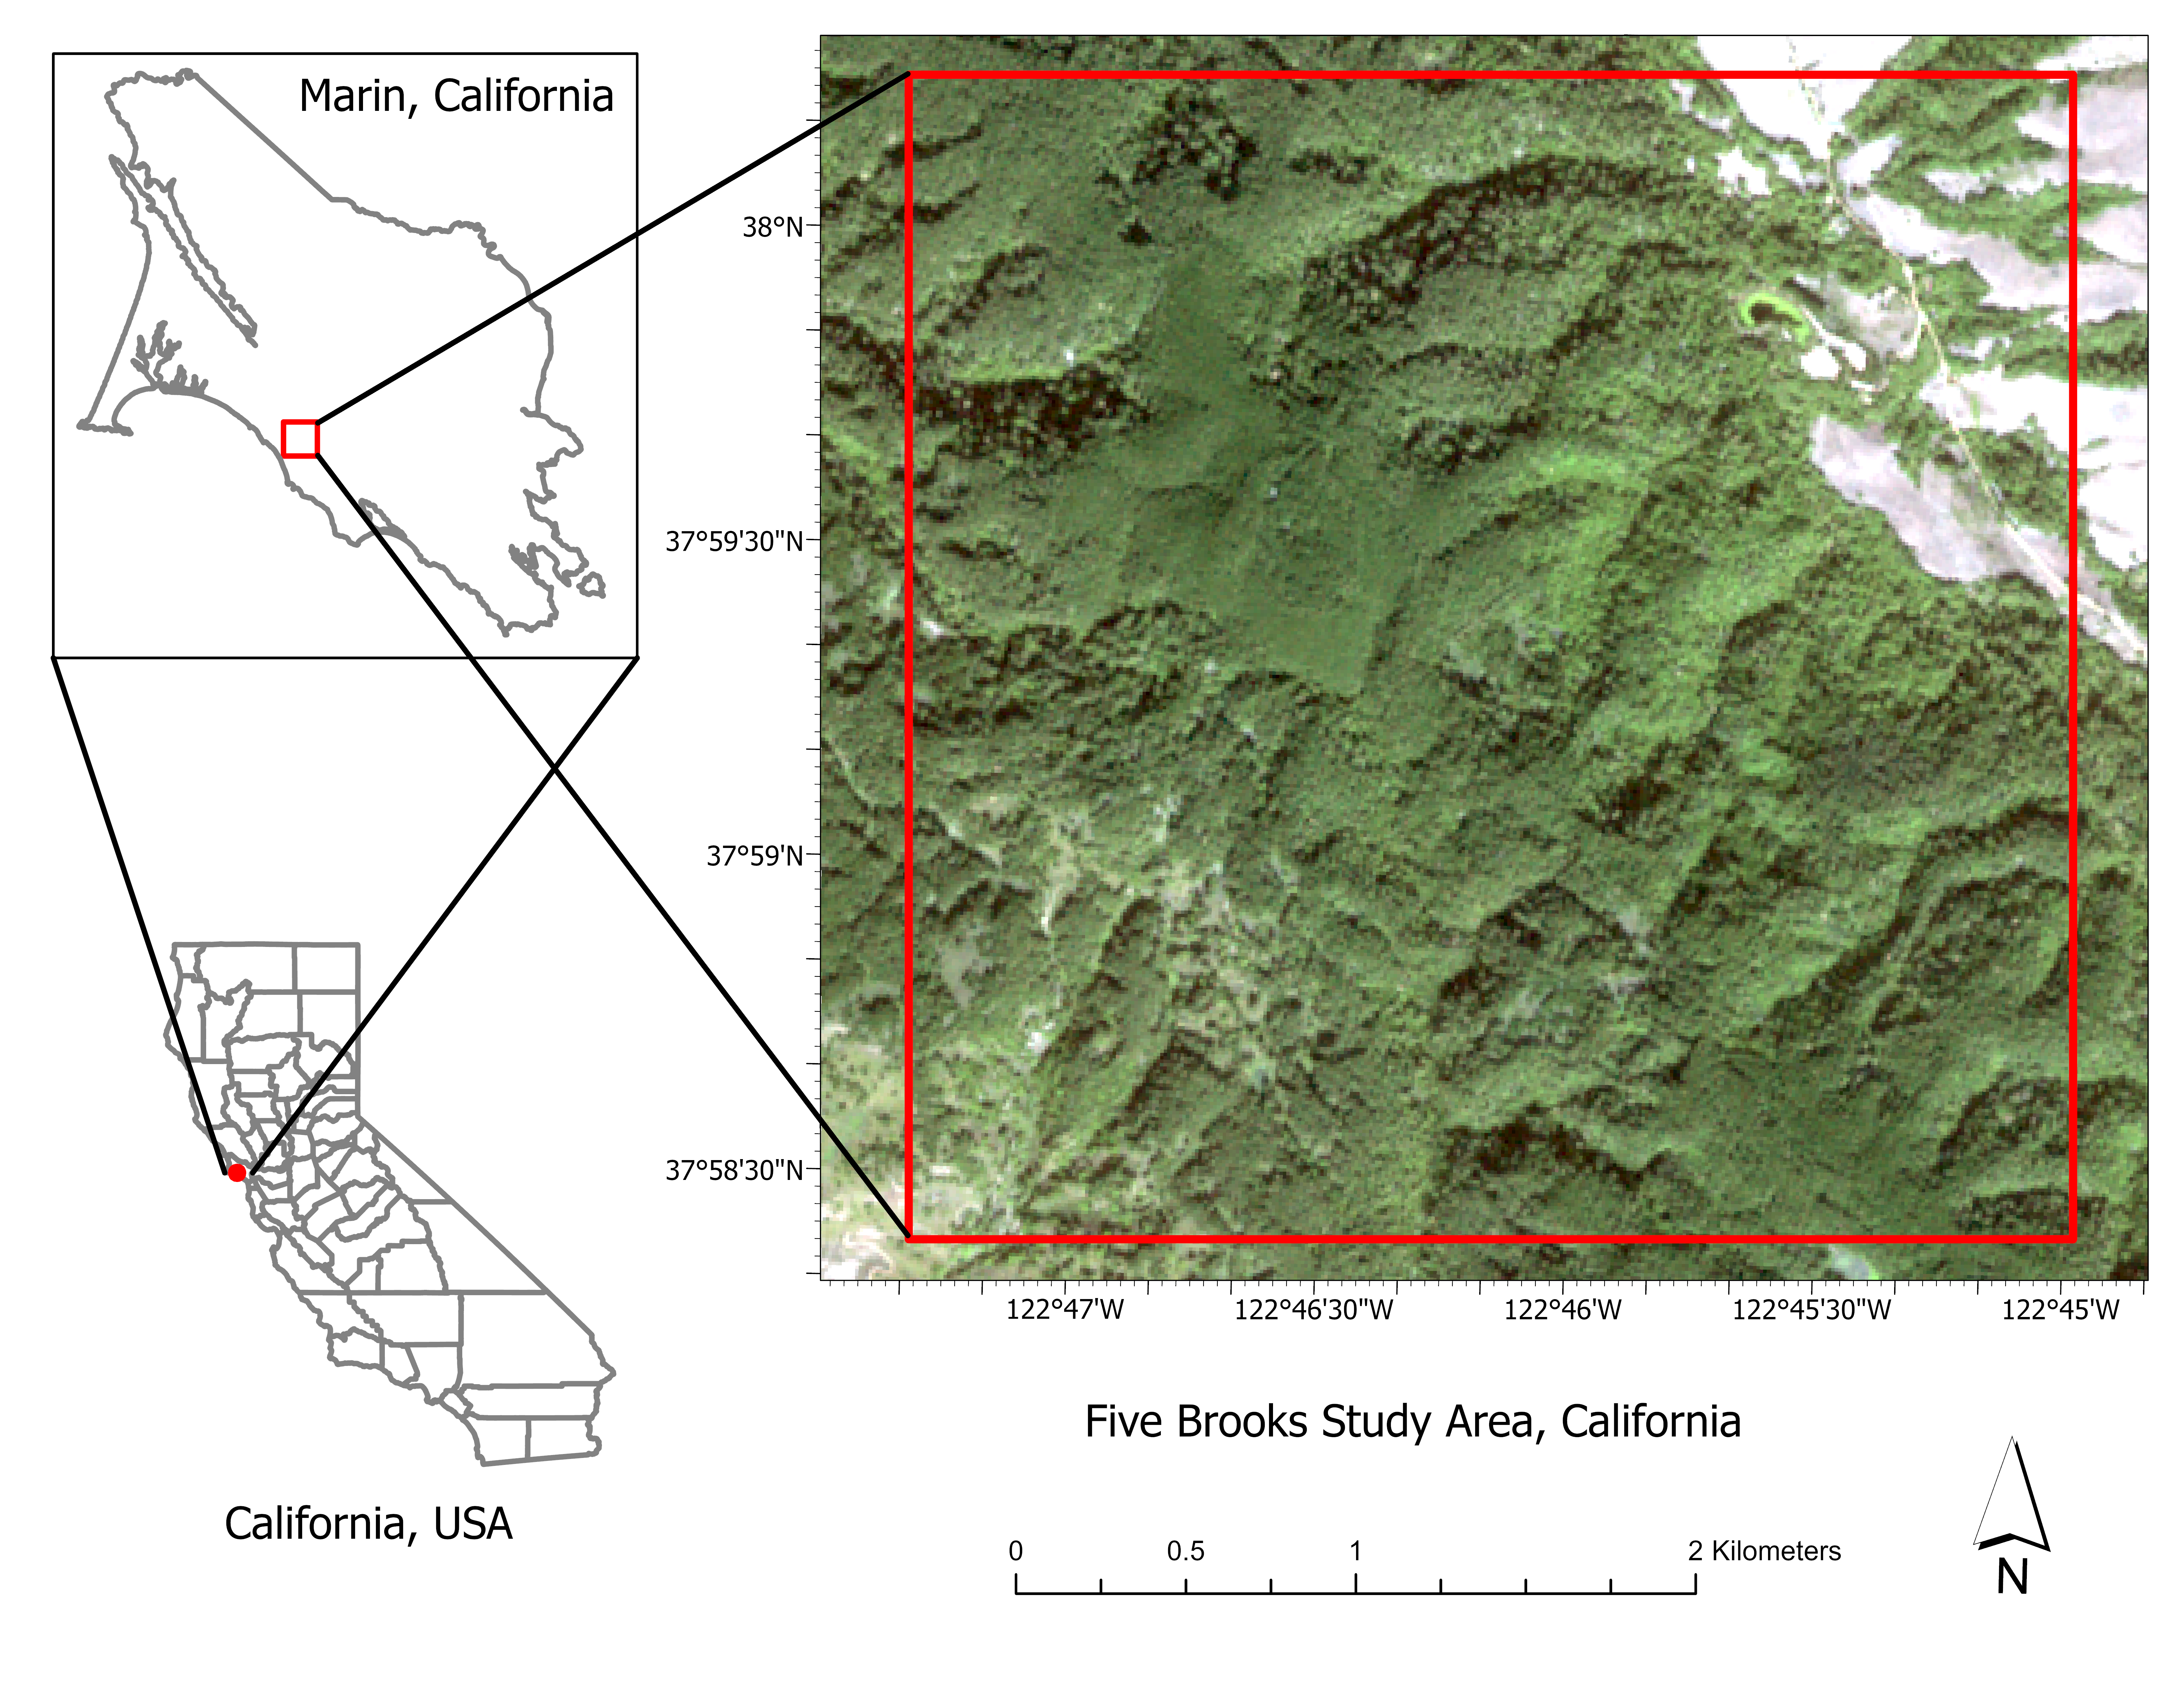
\includegraphics[width=13.7 cm]{LayoutBrooks.png}
\caption{The 11.75 km$^2$ study area is located in the Five Brooks region of the Point Reyes National Seashore. Sentinel 2 imagery from 16 October 2020. \label{fig1}}
\end{figure}  

The first lumber mill in the Point Reyes vicinity was built in Bolinas in 1851. By 1858,~four~mills were operating in the area. Logging continued in Point Reyes until the area was designated a National Seashore in 1962 \cite{livingston}. After the Seashore was established, the logged areas were subsequently left to naturalize \cite{becker}. 

The study area is an area of 11.75 km$^2$ just south of Olema, California and is representative of the logged regions of concern in Point Reyes National Seashore. This area was selected through discussion with National Park Service project leaders, specifically because the area was heavily logged, and no remediation effort has been attempted to decommission the roads \cite{becker}. This site is also the location of ongoing projects by National Seashore managers to understand the lasting effects of historic logging on the region \cite{becker}.

Currently, this area is popular with hikers and has two major trails running through it. The seashore is home to a variety of vegetation from shrubs to trees but is predominately characterized by coastal douglas-fir {\it (Pseudotsuga menziesii var. menziesii)}, coast redwood {\it (Sequoia sempervirens)}, coast live oak {\it (Quercus agrifolia)}, tanoak {\it (Notholithocarpus densiflorus)}, and california bay {\it (Umbellularia californica)}.


\subsection{Types of Roads}
Generally, logging roads within mountainous forested regions fall into two categories: those in a mid-slope position and those that follow or cross over ridge lines \cite{sherba}. Examples of overgrown historic logging roads within the study area shown in Figure \ref{fig2}. Changes in the natural slope of the region are highlighted in red. Figure \ref{fig2}a shows a logging road in a mid-slope position and Figure \ref{fig2}b a road in a ridge-top position. These roads manifest themselves differently in the data, and it is important to recognize that, in order to extract complete road networks, these two road types must be approached separately.

\begin{figure}[H]	
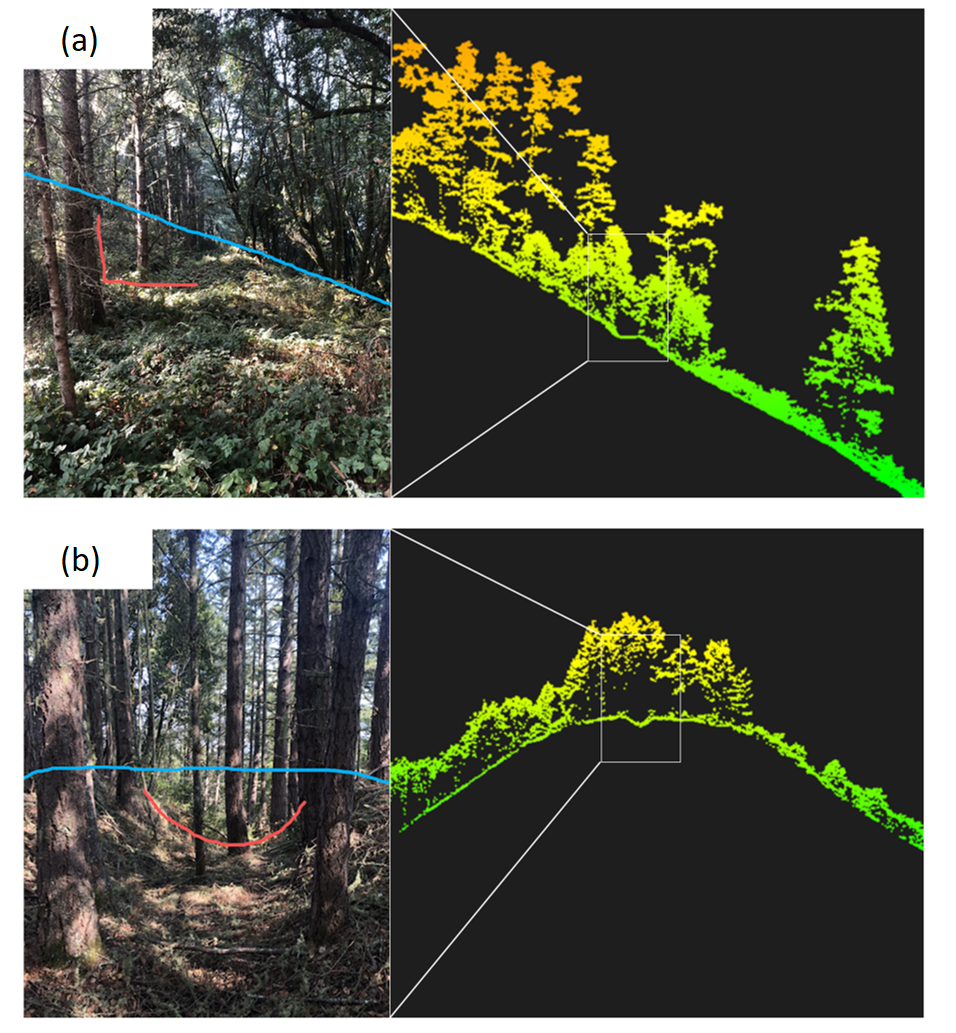
\includegraphics[width=10 cm]{roadtypes.png}
\caption{Two examples of abandoned logging roads present within the study area, where location (\textbf{a}) depicts a sample area within the study area where a road has been placed in a mid-slope position. Location (\textbf{b}) depicts a road in a hill-top position. In photos on left, natural slope is shown in blue, and incised logging roads are marked in red. Graphic on the right depicts cross-sectional views of LiDAR taken of same location.\label{fig2}}
\end{figure}  

\subsection{Data}

LiDAR tiles for Marin County were provided by the Golden Gate National Parks Conservancy \cite{becker}. These tiles have an area of 0.47 km$^2$ each, and the study area comprises exactly 25 complete tiles. The highest resolution LiDAR available for the region was collected by Quantum Spatial between the dates of 22 December 2018 and 15 March 2019 in the format of High-resolution Q1 LiDAR \cite{quantum}. In this file, the average point cloud density of Marin is eight points per m$^2$, However, in the region of the study area the average density is as high as sixteen points per m$^2$. High point cloud density is necessary for an accurate bare earth DEM because a large percentage of the points in a region as densely vegetated as Point Reyes \cite{sherba, white} are absorbed by vegetation %Please check intended meaning has been retained.
.

The LiDAR tiles were mosaicked together in ArcGIS \cite{esri} and then processed into a bare earth DEM from which a slope model was derived. These data were the primary input for the segmentation processes and object-based road identification using eCognition software \cite{ecog}. These steps are covered in subsequent sections.

Historic aerial photos taken of the area in the 1960s were provided by the Point Reyes National Seashore Museum to be used in the accuracy assessment. These photos accurately show the area just after logging ceased \cite{becker}. The aerial photos were scanned at 1200 dpi in a charge-coupled device scanner, converted to 1 m resolution, and georeferenced in ArcGIS. 

Sentinel 2B imagery from 16 October 2020 at a resolution of 10 m (Figure~\ref{fig1}) was chosen to show the current general land cover of the region, although it was not used for analysis because the logging roads have been completely revegetated and are no longer visible using satellite imagery. However, the imagery demonstrates the current state of the region in comparison to the aerial photographs from the 1960s of post-logging, which were used in the accuracy assessment. In the Sentinel 2B imagery, the area can be seen to be completely revegetated with all roads obfuscated from view (Figure~\ref{fig1}). 
\subsection{Data Preparation}

The LiDAR point clouds were downloaded in the form of tiles from the Golden Gate National Parks Conservancy. These LiDAR tiles were then mosaicked together and filtered to only include ground points that have penetrated the canopy and struck ground. Then, a digital elevation model (DEM) was derived from the ground-return-only LiDAR, which was then processed into a slope model.

Logging roads present similarly in the data as, and are often confused with, streams and rivers in slope models \cite{sherba}. Therefore, it was necessary to create a stream layer with which to mask out stream features from analysis. This was achieved by using the DEM derived from the LiDAR to create a flow accumulation raster. It is from this that a stream network was generated, which was used to create a stream order map. This layer was buffered and masked out of the final logging road classification; objects falling within natural drainages were removed from analysis. Shown in Figure~\ref{fig3} are the steps in the road extraction process, which will be covered in the following sections.

\begin{figure}[H]
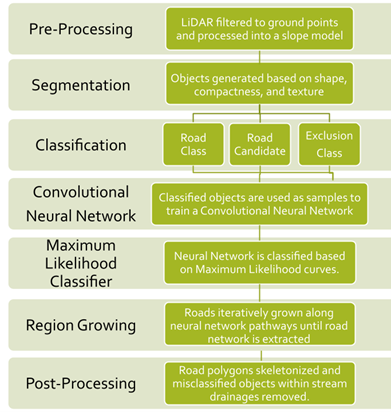
\includegraphics[width=10.5 cm]{workflow.png}
\caption{Workflow from unprocessed LiDAR to extracted road network. \label{fig3}}
\end{figure}    

\subsection{Segmentation}

\textls[-18]{The first step of object-based classification is the image segmentation process, where pixels are aggregated into groups based on their spectral and spatial patterns \cite{alon}. The goal of segmentation is to reduce heterogeneity and increase the homogeneity of image objects \cite{naggar}. The image is broken down into primitive image objects using segmentation algorithms, which cluster pixels together based on their relative spectral value, shape, and texture~\cite{xu}. The exact parameters used in this process can be found in in Appendix \ref{appendix:a}. Using these primitive image objects, features within the scene can then be extracted \cite{naggar, xu}. Multi-resolution segmentation, within eCognition, has been shown to be one of the most effective methods to categorize complex landscape features into meaningful objects \cite{carreira, naggar, tab}. However, the scale, shape, and compactness parameters are typically determined in a heuristical manner. Scale refers to the size of image objects relative to the scene’s resolution \cite{duan, naggar}. Generally, to avoid over-segmentation or under-segmentation, a scale should be chosen that results in image objects that encompass the entirety of what is being attempted to classify \cite{duan, sherba}. Shape has two components: smoothness and compactness. Smoothness refers to the roughness of the edges of the image objects, and compactness refers to the object’s length versus width \cite{naggar}. For this research, a weight of 0.1 for shape, a compactness of 0.8, and a scale of 11 were found to be the best for this particular site under these particular conditions %Please check intended meaning has been retained. !Yes, this is good thank you -W
. These numbers, which were arrived at manually, are data-scale-dependent, and if this workflow were applied to LiDAR of a different quality or to a region whose morphology presented in a significantly different way, it is likely that these numbers would have to be adjusted. It is important to remember that the goal of image segmentation is to break an image into homogeneous objects and that specific parameter weights are dependent on the range of values present in the input raster, as well as that raster’s resolution. In this situation, we are particularly interested in arriving at objects that span the complete width of the roads (Figure~\ref{fig4}). Segments that span the entire width of the object being classed can gather the spectral and spatial information of neighboring objects in OBIA \cite{duan, sherba, xu}. Within the study area, objects encompassing undisturbed hillslope areas have a higher slope value than roads that have been graded for logging equipment. With objects that span the entire width of the low-sloped roads, it is possible to use the contextual information from neighboring high-sloped objects in the classification of the road objects. }
\begin{figure}[H]
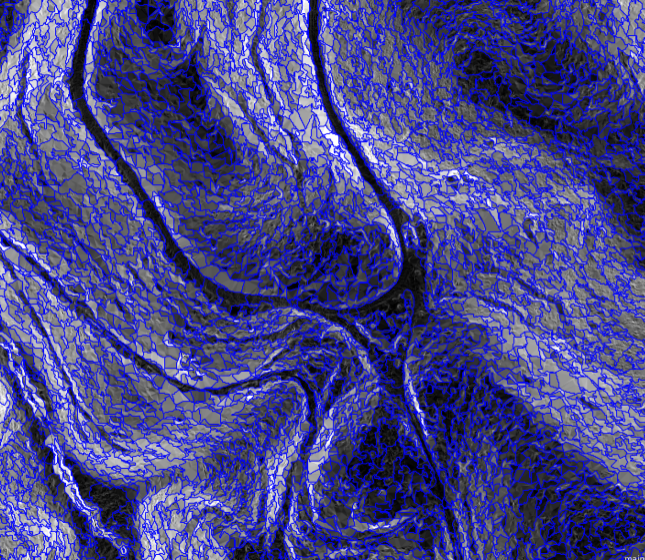
\includegraphics[width=10.5 cm]{segment.png}
\caption{A small subset of the training area after segmentation.  \label{fig4}}
\end{figure}   


\subsection{Initial Classification and Region Growing}


For this research, we considered two zones: one training-zone, for training the CNN-model, and one validation zone for applying the model to assess its performance independently of the training \cite{navulur, prakash}. The validation area was only used for the accuracy assessment stage of this study and was chosen from where there was historic aerial photo coverage that could be accurately georeferenced. The training area was chosen based on its coverage of different types of terrain and roads to ensure that road types from a variety of environmental conditions would be included in the model.

Road objects were classified based not only on their own spectral signature but also the signature of their neighbors, and other relationships such as size and shape. As depicted in Figure \ref{fig2}, the position of roads in the landscape determines how they can be detected in a slope model. Roads in a mid-slope position in most cases are of a low slope and bordered on either side by high slopes (Figure~\ref{fig2}a). After classification, these initial road objects were expanded to encompass neighboring objects using region growing algorithms %Please check intended meaning has been retained.
.

Region growing is a method to classify image objects by first identifying a seed object within the segmented image and then growing this seed into the desired segmented object through iterations of growing and merging regions \cite{benz}. In some road detection applications, it is known where the objects to be classified are located \cite{li}, which aids in the seeding process. This is typically followed by multiple iterations of region growing until the objects are classed. However, because not only the initial seed location must be known but also when to stop the region growing, this requires significant expert knowledge of the region to be classified. This can be the most difficult part of creating an automated system of classification.

In the case of abandoned logging roads, there are two additional problems: (1) it is not known where all of the logging roads are located, and (2) the logging roads are highly fragmented and may no longer be connected due to changes in the geomorphology of the region. The latter point becomes a prohibitive complication if not every road fragment is seeded during the initial steps of the process \cite{li}. This process of seeding and growing is time consuming, can have a number of parameters to adjust, lacks standardized documentation, and can require significant time to develop effective methods %Please check intended meaning has been retained.
~\cite{idrees}. 

However, the object identification and seeding process can be fully automated through identifying specific features unique to the objects.   Road features are more   subtle than other types of objects extracted in OBIA, and the highly pronounced features typically utilized to automatically seed the region are not present. Because of this, it is required to use the almost imperceptible changes in the terrain that might be detectable in a slope model \cite{luca, erikson, sherba, zhen}.

For this study, three classifications of the objects within the scene were used. Objects with a very high slope are not roads, and therefore these were assigned to the (1) ‘exclusion’ class. Next, all other objects within the scene were assigned to the (2) ‘candidate’ class, which may or may not be a road. Then, these candidate objects,   which had a low slope but were bordered on either side by high slope, were classified as the (3) ‘road’ class. These road objects were then grown into   neighboring candidate objects with a similar slope. Roads that were not captured by the road class ruleset were classified by their road-based slope characteristics and their connectivity to roads; road seed objects that had a high certainty of being roads were grown iteratively along low slope road pathways into areas of less certainty.   This method was utilized to avoid the miss-classification of other low-slope areas %Please check intended meaning has been retained.
(such as hilltops) as roads.  

Complete coverage of all road objects was not achieved through this process, although a sampling of road objects from many different environments (hilltop and mid-slope) was found.  In general, neural networks are most successful if the dataset has a sampling of objects to be classified across the entirety of the environments in which they are present~\cite{prakash}. These objects were then used as input samples to train the CNN machine learning algorithm.  

\subsection{Training and Applying the CNN}
The road objects from the training subset were used as the input samples in a CNN~\cite{ecogcnn}. The first 1000 samples points for each class (road, candidate, and exclusion) were taken from within their classified image objects. Then, the canvas was rotated by 30 degrees and another 1000 samples were taken for each class. This process was repeated iteratively until the map returned to the start after 12 cycles. This rotation was implemented to increase the number of samples, as well as to ensure that the resulting CNN did not spatially correlate the sample points to one another. This resulted in a total of 36,000 samples (12,000 for each class). This was then used to make a 3-layer convolutional neural network, consisting of a convolutional, a pooling, and a fully connected layer. The convolutional layer is where features from the input to the CNN were extracted. The pooling layer then reduced the spatial volume of input image. The fully connected layer connected neurons in one layer to neurons in another layer to classify the image, where the neurons are computational units designed to find patterns in the pooling layer and whose numbers represent the number of pixels in the input image \cite{prakash}.

The output of the CNN was one prediction layer for each input class in the form of a heatmap. A heatmap displays the magnitude of a phenomenon; in the case of CNNs, the values of the resulting heat maps directly represent the model’s prediction of the probability (from 0 to 1) of that class being present in a given area \cite{prakash, timilsina}. The resulting heat maps from the CNN were then used as an input to guide the classification of the image segments.
 
Shown in Figure~\ref{fig5} is the resulting output of the convolutional neural network in the validation area. The CNN created a one band heatmap for each of the three class types; these outputs were then stacked into a 3-band raster stack with each band (red, blue, and green) corresponding to a classification parameter (road, candidate, and exclusion). This raster stack is for visualization purposes to better understand and conceptualize the region being analyzed. This visualization’s purpose is to highlight areas with a high confidence of being roads compared to areas of exclusion or uncertainty.

\begin{figure}[H]
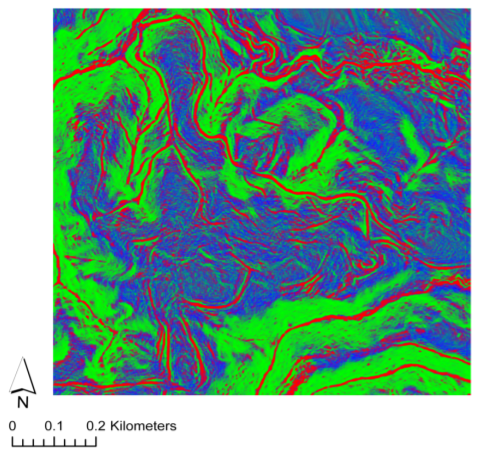
\includegraphics[width=12 cm]{cnn.png}
\caption{The output of the convolutional neural network. Each color band corresponds to each one of the three classes present in the model. Red represents the areas of highest likelihood of being roads (road class); blue represents possible roads (candidate class); and green highest likelihood of not being roads (exclusion class). \label{fig5}}
\end{figure}  

\subsection{Classifying and Extracting the Road Network}

To reclassify the CNN, a threshold was set in the heatmap from which the features were extracted \cite{luca, prakash, timilsina}. These thresholds were extracted using the maximum likelihood classifier, which designated which class an object in the scene belongs to. The maximum likelihood classifier calculates the probability that a given object belongs to a specific class based on defined membership curves, with the value of the object being the mean of the pixels contained within it \cite{richards}. The fine-tuned membership function curves can be seen in Figure~\ref{fig6}. An object was attributed to a specific class based on the highest value of the averaged pixels within the image object of the corresponding layer (road, candidate, and exclusion) as defined by the CNN. Using this method, image segments with higher road heatmap values associated with them were classified as road, segments associated with the exclusion zone were classified as excluded, and candidates as candidates %Please check intended meaning has been retained.
. Each object is assigned to the class that has the highest presence within the object. Image segments between these classes were classified based on the likelihood that they might belong to one class or another based on these curves (Figure~\ref{fig6}). These objects were then used to re-seed the image.
\vspace{-6pt}
\begin{figure}[H]
\begin{adjustwidth}{-\extralength}{0cm}
\centering
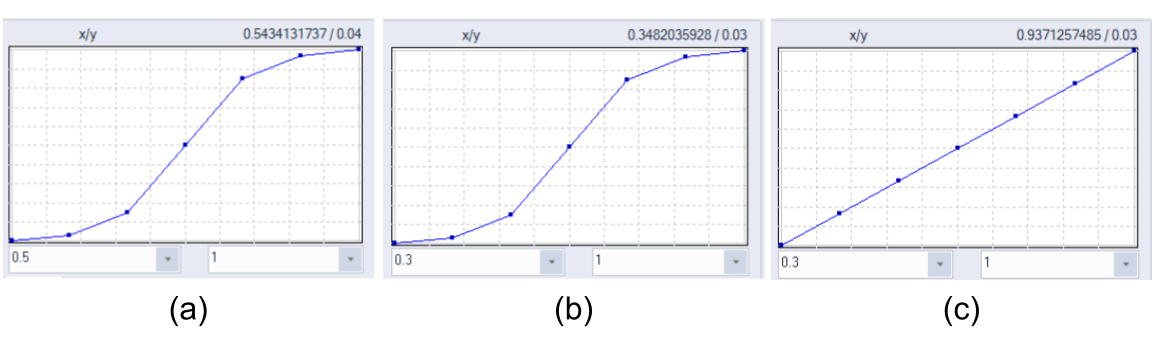
\includegraphics[width=17cm]{membership.png}
\end{adjustwidth}
\caption{Membership functions in eCognition for maximum likelihood classifier from CNN heatmaps, where item (\textbf{a}) shows road membership, item (\textbf{b}) depicts the candidate class for growing roads into, and item (\textbf{c}) shows the exclusion class. \label{fig6}}
\end{figure}  

After classification, road seed objects were grown iteratively along the pathways of the CNN to fill in classification gaps and identify hilltop roads until the network had been fully extracted. Since the CNN better identified road objects that were not evident in the slope model, a more complete and better connected road network could be obtained. Figure~\ref{fig7} illustrates the process of extracting this more complete road network. Figure~\ref{fig7}a shows the initial segmentation, Figure %MDPI: We changed it to figure citation, please confirm. !This is fine with me, thank you -W
\ref{fig7}b depicts the initial classification, Figure~\ref{fig7}c shows the trained neural network's output, and Figure~\ref{fig7}d shows the growing process along the neural network~pathways. 

\begin{figure}[H]
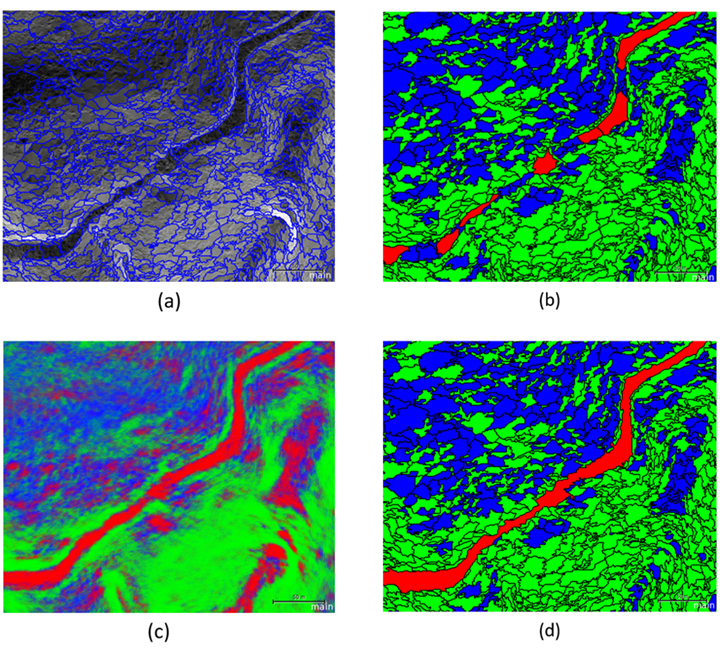
\includegraphics[width=12 cm]{classify.png}

\caption{ The road classification process, where (\textbf{a}) shows initial segmentation, item (\textbf{b}) depicts initial classification, item (\textbf{c}) shows the trained neural network's output, and item (\textbf{d}) shows the growing process along neural network pathways. In items (\textbf{b}) through (\textbf{d}), red represents the areas with the highest likelihood of being roads (road class); blue represents possible roads (candidate class); and green represents the highest likelihood of not being roads (exclusion class).}\label{fig7}
\end{figure}

Next, an iterative growing and shrinking step was added to smooth the road network and prepare it for extraction. This resulting model included both roads and rivers, but this was to be expected in this type of model \cite{sherba}, and therefore rivers were masked out using the stream order network described in the data preparation stage. In a final step, the road network polygons were skeletonized (the centerline of a polygon) into a line type road-network and exported to a shapefile \cite{lewandowicz}. 
\subsection{Accuracy Assessment}


For an accuracy assessment in remote sensing studies, often the most common technique used is a ground survey, where the ground truthing is found through on-the-ground surveys and compared to the classified map. However, many of the logging roads in this project were so overgrown that accessing and verifying them on the ground was difficult or impossible. Historic aerial photos are a suitable alternative to ground surveys, especially when the features being classed can be reliably extracted from imagery. Aerial photos also have the benefit of being a form of remotely sensed data that can be processed off site, which lowers costs and effort \cite{lillesand}.  

In the case of abandoned logging roads, aerial photographs are an acceptable source of information on the state of the post-logging landscape. Aerial photos of the Point Reyes National Seashore from 1963 document the area just after logging had ceased \cite{becker}. The photos were georeferenced, and the road network was overlain and buffered with a 15~m corridor as a tolerance due to possible geometric errors \cite{zhen}. Any accuracy assessment points falling within this buffer were considered a road. 

Accuracy assessments consider misclassified points as either errors of omission (where a point is classified as non-road within the road network) or errors of commission (a point being classified as road outside of the road network) \cite{lillesand}. These errors were considered in the aerial imagery where vegetation had previously been removed and road/non-road areas could be clearly seen. The aerial photos post logging still had some small areas obscured from view and therefore could not be vectorized properly in those regions. In these areas, where there was uncertainty as to the validity of the classified points, ground surveys were used instead. Thus, ground surveys were used in two instances: (1) the roads were obscured by vegetation, or (2) there was not photo coverage.

This accuracy assessment only considered two classes: road and non-road.  A total of 500 accuracy assessment points were taken across these two classes within their feature areas \cite{guillen, lillesand}. A stratified random accuracy assessment was utilized where points were randomly distributed within each class and where each class had a number of points proportional to its relative area \cite{foody}. Errors of omission and commission were calculated, with the final result being a confusion matrix whose values were used to calculate accuracy and precision.
%%%%%%%%%%%%%%%%%%%%%%%%%%%%%%%%%%%%%%%%%%
\section{Results}
Depicted in Figure~\ref{fig8} is the extracted road network overlain over a historic aerial photo of the region that was used for the accuracy assessment. Through simple visual inspection, these road networks can still be reliably seen despite ~60 years of naturalization.  

\begin{figure}[H]
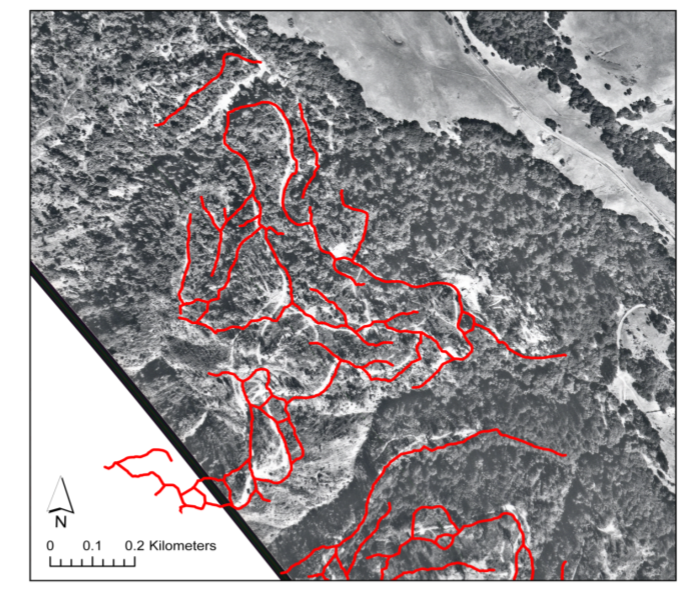
\includegraphics[width=11 cm]{roads.png}
\caption{The extracted road network overlain over a historic aerial photo of the region that was used in the accuracy assessment. \label{fig8}}
\end{figure} 

This research successfully extracted a significant, vast majority of the forest roads within the study area. Within the validation area, a total of 25.725 km of roads were extracted within a 1 km$^2$ area. 

The confusion matrix results from the accuracy assessment are found in Table \ref{tab1}. Formulas used for calculating accuracy and precision can be found in Table \ref{tab2}. For this area, a Kappa of 0.977 (Table \ref{tab1}), a precision of 0.991, and an accuracy of 0.992 were found (Table \ref{tab2}). Kappa values generally have been falling out of favor in the remote sensing community, with a variety of other metrics taking their place \cite{guillen} (as shown in Table \ref{tab2}). Many recent image-analysis papers have adopted using confusion matrix formulas in their results \cite{foody, guillen, papp, prakash, sivakumar, yang}. Since there is a lack of standardization between studies, to allow for comparison, all standard formulas have been included here.

%%%
\begin{table}[H]
\caption{Confusion %MDPI: We revised alignment and border line, please confirm. !I confirm that this looks good to me, thank you -W
 matrix from accuracy assessment.}
\label{tab1}
\newcolumntype{C}{>{\centering\arraybackslash}X}
\begin{tabularx}{\textwidth}{CCCCCC}
\toprule
 & \textbf{Roads} & \textbf{Non-Roads} & \textbf{Total} & \textbf{Accuracy} & \textbf{Kappa}  \\ 
\midrule
\text{Roads} & 112 & 1 & 113 & 0.99115 \\
\midrule
\text{Non-Roads} & 3 & 384 & 387 & 0.99225 \\
\midrule
\text{Total} & 115 & 385 & 500 &  \\
\midrule
\text{Accuracy} & 0.97391 & 0.99740 &  & 0.992  \\
\midrule
\text{Kappa} & & & & & 0.97728 \\
\bottomrule
\end{tabularx}
\end{table}

\vspace{-12pt}
% \usepackage{rotating}
%\begin{sidewaystable}
\begin{table}[H]
\caption{Formulas %MDPI: We revised alignment and border line, please confirm. !I confirm that I am happy with this table, thank you -W
 for understanding the confusion matrix results. TP = true positive, TN = true negative, FP = false positive, and FN = false negative.}
\label{tab2}
\begin{adjustwidth}{-\extralength}{0cm}
		\newcolumntype{C}{>{\centering\arraybackslash}X}
		\begin{tabularx}{\fulllength}{CCc}
\toprule
 \textbf{Measure} & \textbf{Value} & \textbf{Derivations}  \\ 
\midrule
\text{Sensitivity} & 0.9739 & TPR = TP/(TP + FN) \\
\midrule
\text{Specificity} & 0.9974 & SPC = TN/(FP + TN)  \\
\midrule
\text{Precision} & 0.9912 & PPV = TP/(TP + FP)   \\
\midrule
\text{Negative Predictive Value} & 0.9922 & NPV = TN/(TN + FN)   \\
\midrule
\text{False Positive Rate} & 0.0026 & FPR = FP/(FP + TN) \\
\midrule
\text{False Discovery Rate} & 0.0088 & FDR = FP/(FP + TP) \\
\midrule
\text{False Negative Rate} & 0.0261 & FNR = FN/(FN + TP) \\
\midrule
\text{Accuracy} & 0.9920 & ACC = (TP + TN)/(TP + TN + FP + FN) \\
\midrule
\text{F1 Score} & 0.9825 & F1 = 2TP/(2TP + FP + FN) \\
\midrule
\text{Matthews Correlation Coefficient} & 0.9773 & TP*TN %MDPI: Please check if * should be changed to multiplication sign (× $times$). !yes this is how its referred to in the primary literature.
 $-$ FP*FN/sqrt((TP + FP)*(TP + FN)*(TN + FP)*(TN + FN)) \\
\bottomrule
\end{tabularx}
	\end{adjustwidth}
\end{table}
%\end{sidewaystable}
%%%


%%%%%%%%%%%%%%%%%%%%%%%%%%%%%%%%%%%%%%%%%%
\section{Conclusions}

The goal of this study was to extract historic forest road networks out of LiDAR point clouds under heavy canopy. This work attempted to augment the currently used automated road extraction process to better capture hilltop roads and fill gaps in cutbank roads by investigating the use of CNNs to automate and improve OBIA accuracy.

The results have shown that roads were able to accurately be identified in LiDAR using OBIA in conjunction with CNNs. Specifically, the results show that OBIA methods can be improved upon using CNNs. CNNs help to increase classification accuracy and automate the extraction methods that, in previous research, had to be processed using non-autonomous methods. The results of this study’s coupled CNN, OBIA approach have minimized these errors, improved classification accuracy, and captured hilltop roads.

When looking at studies of similar areas, such as Sherba et al. \cite{sherba}, %Please cite reference with reference numbers, and place the numbers in square brackets [ ], for example [1], [1-3] or [1,3], You may refer to the following the website: http://www.mdpi.com/authors/references. !This has been updated thank you -W
 pixel-based classification results show that the unsupervised classification of logging roads had a total accuracy of 78\%. They also found that the errors of commission occurred largely on ridgelines where large areas of low slope were present, and errors of omission occurred as gaps in the road network \cite{sherba}. In their paper, when a strictly fully automated OBIA approach was used, an initial classification accuracy of 86\% was found. Additionally, after extracting out misclassified drainages and incorporating in hand-digitized ridge roads, classification accuracy increased to 90\%.

Sherba et al. \cite{sherba} classified their segmented slope model into two initial classes: roads that were considered ‘certain road objects’, and ‘road candidate objects’, which were roads only if they were near the initial road class. They then grew these road objects into the candidate object class to create a logging road map \cite{sherba}. A major difficulty in this workflow was the time-consuming nature of the task and the lack of automation in its identification of hilltop roads. In order to increase the practicality of road extraction methods, this research effort has also added an exclusion class (of areas certain not be roads) to restrict the possibility of roads growing into areas with an extremely low likelihood of being roads.

This work incorporates their OBIA process with CNN machine learning techniques. First, OBIA was used to carry out an initial classification of the region; then, these objects were used as samples for a CNN machine learning algorithm. The output of the CNN was then used to re-segmented the image. Next, the resulting segmentation was classified based on the maximum likelihood classifier, from which the road network was extracted. This process increased classification accuracy, automated the process of identifying hilltop roads, and aided the process of filling in gaps in hillside roads.

Some novel findings of this research are:
\begin{enumerate}[]
\item In order to segment a slope raster, objects should completely span roads because this allows for the incorporation of neighboring objects of, for example, higher slope values to be used in the classification of road objects.

\item When attempting to expand the road network through the growth road-classified image objects, the low slope of the road can be used, but this is greatly improved upon by using the values contained in the roads CNN.  

\item Road objects and stream objects are almost identical. At this stage, it is recommended to mask out these objects during post-processing. Although an automated process to remove these is desirable, more research is needed.

\item The output of the CNN appears to highlight road objects that may be producing more sediment. Proportional road surface area has been shown to be positively correlated to sediment discharge \cite{reid}. The heatmaps resulting from the CNN empirically appear to be associating higher road values with road objects of a greater surface area. Future research is needed to understand if the road features in the CNN that have higher values associated with them are producing more sediment and should have a higher remediation priority. If this is true, it may be possible to adapt the CNN algorithm to make a ‘road order’ map of road objects that have the greatest impact on streams in the region. To achieve this objective, more field research would be needed in the measuring of sediment loads being produced from these features.  
\end{enumerate}

%%%%%%%%%%%%%%%%%%%%%%%%%%%%%%%%%%%%%%%%%%
\vspace{6pt} 




\authorcontributions{Author Contributions: William Wiskes conceptualized and designed the study, conducted the research, analyzed the data, and wrote the manuscript. Leonhard Blesius and Ellen Hines provided guidance and critical feedback throughout the research process and contributed to the editing and revision of the manuscript} %For research articles with several authors, a short paragraph specifying their individual contributions must be provided. The following statements should be used "Conceptualization, X.X. and Y.Y.; methodology, X.X.; software, X.X.; validation, X.X., Y.Y. and Z.Z.; formal analysis, X.X.; investigation, X.X.; resources, X.X.; data curation, X.X.; writing---original draft preparation, X.X.; writing---review and editing, X.X.; visualization, X.X.; supervision, X.X.; project administration, X.X.; funding acquisition, Y.Y. All authors have read and agreed to the published version of the manuscript.'', please turn to the  \href{http://img.mdpi.org/data/contributor-role-instruction.pdf}{CRediT taxonomy} for the term explanation. Authorship must be limited to those who have contributed substantially to the work~reported}. 
 %please ensure all authors have been stated

\funding{This research received no external funding.}

\dataavailability{The proprietary nature of the data prevents us from publicly archiving or sharing it at this time. Interested researchers may request access to the data from the Golden Gate National Parks Conservancy. Details on how to obtain access to the data can be obtained by contacting the organization directly. The methodology employed in this study is provided in the Appendix section of the paper.} %We encourage all authors of articles published in MDPI journals to share their research data. In this section, please provide details regarding where data supporting reported results can be found, including links to publicly archived datasets analyzed or generated during the study. Where no new data were created, or where data is unavailable due to privacy or ethical re-strictions, a statement is still required. Suggested Data Availability Statements are available in section “MDPI Research Data Policies” at \url{https://www.mdpi.com/ethics}.} 

\acknowledgments{I would like to thank Shawn Maloney of Point Reyes National Seashore for his help in organizing the project and his input in the selection of the study area. I would like to thank Paul Engel of Point Reyes National Seashore for his help with accessing the museum containing the historic photos, as well as his help with finding the proper photos for the study region. Moreover, I would like to thank Ben Becker of the Point Reyes National Seashore for his help with organizing the project.}

\conflictsofinterest{The authors declare no conflict of interest.} 

\abbreviations{Abbreviations}{
The following abbreviations are used in this manuscript:\\

\noindent 
\begin{tabular}{@{}ll}
CNN & Convolutional neural network\\
LiDAR & Light detection and ranging\\
OBIA & Object-based image analysis\\
DEM & Digital elevation model
\end{tabular}
}

%%%%%%%%%%%%%%%%%%%%%%%%%%%%%%%%%%%%%%%%%%
%% Optional
\appendixtitles{yes} 
\appendixstart
\appendix
\section[\appendixname~\thesection]{Process Tree}\label{appendix:a} %MDPI: !!! Please cite Appendix A in the main text. !This task is now complete -W


 %Please check intended meaning has been retained. !Sentence has been moved to figure caption -W
%MDPI: Please add figure caption for the two images below if possible, i.e., Figure A1. xxx.  Figure A2. xxx. !They are really both the same figure so I have combined them and added one caption -W
\begin{figure}[H]
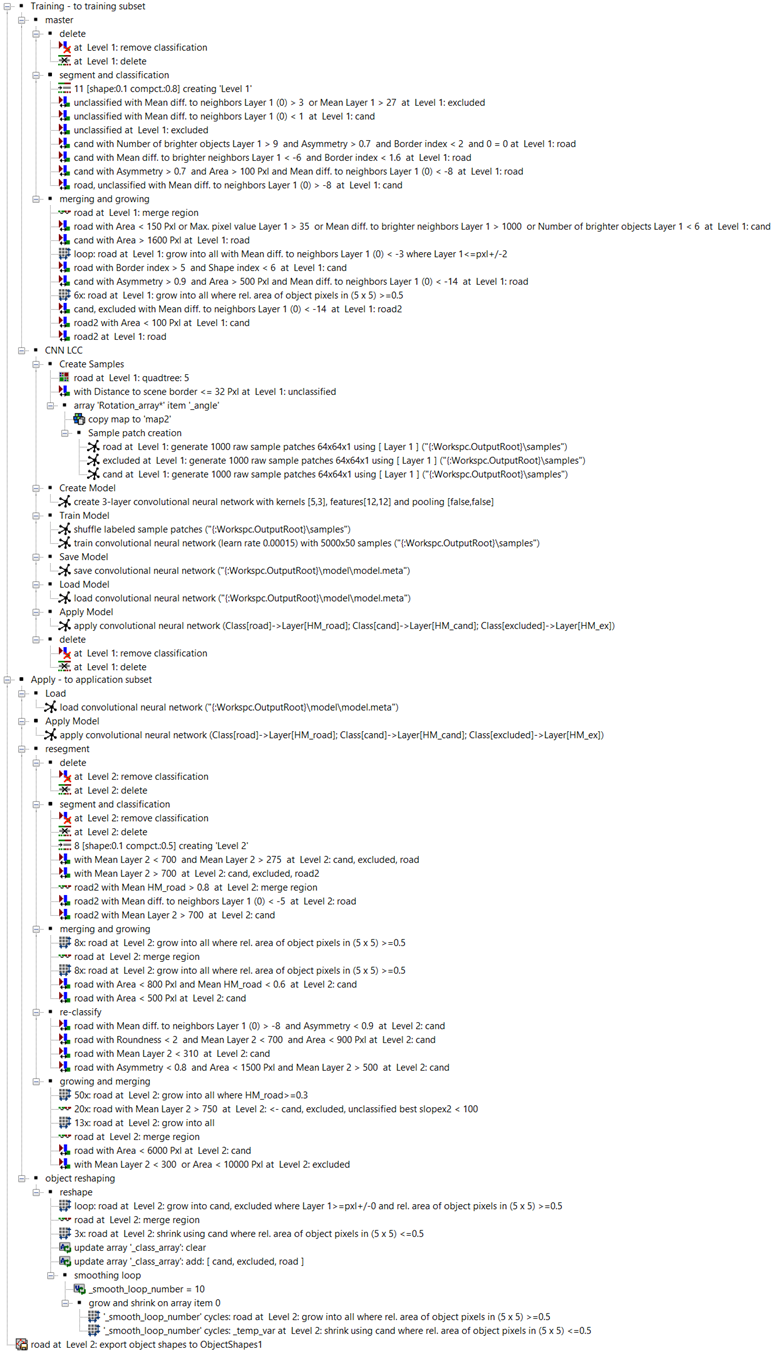
\includegraphics[width=12 cm]{appendix.png}
\caption{Complete eCognition process tree to extract the road network. \label{figA}}
\end{figure}   
\newpage

%%%%%%%%%%%%%%%%%%%%%%%%%%%%%%%%%%%%%%%%%%
\begin{adjustwidth}{-\extralength}{0cm}
%\printendnotes[custom] % Un-comment to print a list of endnotes

\reftitle{References}




\begin{thebibliography}{999}

\bibitem[Becker and Maloney(2020)]{becker}
Becker, B. (National Park Service, Point Reyes, USA); %MDPI: please add his Affiliation !complete -W
Maloney, S.  (National Park Service, Point Reyes, USA). %MDPI: please add his Affiliation !complete -W
\newblock Personal communication, %%MDPI: please delete it !complete -W
2020. 
%MDPI: for Personal Communications type reference, please write it with the format: 
%Author 1 (Affiliation 1); Author 2 (Affiliation 2). Personal communication, Year. 
%For example,
%Heinonen, J. (Aalto University, City, Country); Mattila, T. (Finnish Environment Institute, City, Country). Personal communication, 2012.



\bibitem[Sherba et~al.(2014)Sherba, Blesius, and Davis]{sherba}
Sherba, J.; Blesius, L.; Davis, J.
\newblock Object-Based Classification of Abandoned Logging Roads under Heavy
  Canopy Using LiDAR.
\newblock {\em Remote Sens.} {\bf 2014}, {\em
  6},~4043--4060.
\newblock https://doi.org/10.3390/rs6054043.

\bibitem[White et~al.(2010)White, Dietterick, Mastin, and Strohman]{white}
White, R.A.; Dietterick, B.C.; Mastin, T.; Strohman, R.
\newblock Forest Roads Mapped Using LiDAR in Steep Forested Terrain.
\newblock {\em Remote Sens.} {\bf 2010}, {\em
  2},~1120--1141.
\newblock https://doi.org/10.3390/rs2041120.

\bibitem[Rab(2004)]{rab}
Rab, M.A.
\newblock Recovery of soil physical properties from compaction and soil profile
  disturbance caused by logging of native forest in Victorian Central
  Highlands, Australia.
\newblock {\em For. Ecol. Manag.} {\bf 2004}, {\em 191},~329--340.
\newblock https://doi.org/10.1016/j.foreco.2003.12.010.

\bibitem[Troendle and King(1985)]{troendle}
Troendle, %MDPI: We removed website link since it's not required in journal type, please confirm. !cofirming this is ok -W
 C.A.; King, R.M.
\newblock The Effect of Timber Harvest on the Fool Creek Watershed, 30 Years
  Later.
\newblock {\em Water Resour. Res.} {\bf 1985}, {\em 21},~1915--1922. https://doi.org/10.1029/WR021i012p01915.

\bibitem[Luce and Black(1999)]{luce}
Luce, %MDPI: We removed website link since it's not required in journal type, please confirm. !cofirming this is ok -W
 C.H.; Black, T.A.
\newblock Sediment production from forest roads in western Oregon.
\newblock {\em Water Resour. Res.} {\bf 1999}, {\em 35},~2561--2570. https://doi.org/10.1029/1999WR900135.

\bibitem[Underwood(2009)]{underwood}
Underwood, K.R.
\newblock (2009). The Effects of Hillslopes on Trail Degradation Olympic National Park, Washington. University of Arkansas, Fayetteville. %MDPI: Please provide more information about the article type, such as book (please provide the name and location of the publisher); online resource (please provide the URL of the website and the date it was accessed (Date Month Year)); or journal article (please provide the name of the journal, the year and volume in which it was published, and the page number). Please refer to https://www.mdpi.com/authors/references for full reference formatting guides.
% !complete -W
% @book{underwood2009effects,
%   title={The Effects of Hillslopes on Trail Degradation Olympic National Park, Washington},
%   author={Underwood, K.R.},
%   url={https://books.google.com/books?id=TRU9QwAACAAJ},
%   year={2009},
%   publisher={University of Arkansas, Fayetteville}
% }


\bibitem[Douglas et~al.(1992)Douglas, Spencer, Greer, Bidin, Sinun, and
  Meng]{douglas}
Douglas, I.; Spencer, T.; Greer, T.; Bidin, K.; Sinun, W.; Meng, W.W.
\newblock The Impact of Selective Commercial Logging on Stream Hydrology,
  Chemistry and Sediment Loads in the Ulu Segama Rain Forest, Sabah, Malaysia.
\newblock {\em Philos. Trans. Biol. Sci.} {\bf 1992},
  {\em 335},~397--406. https://doi.org/10.1098/rstb.1992.0031.

\bibitem[Wemple et~al.(2001)Wemple, Swanson, and Jones]{wemple}
Wemple, B.C.; Swanson, F.J.; Jones, J.A.
\newblock Forest roads and geomorphic process interactions, Cascade Range,
  Oregon.
\newblock {\em Earth Surf. Process. Landforms} {\bf 2001}, {\em
  26},~191--204. https://doi.org/10.1002/1096-9837(200102)26:2<191::AID-ESP175>3.0.CO;2-U.

\bibitem[Wong and Neo(2019)]{wong}
Wong, K.; Neo, L.
\newblock Species richness, lineages, geography, and the forest matrix:
  Borneo's `Middle Sarawak' phenomenon. {\em Gard. Bull. Singap.} {\bf 2019}.
\newblock {\em 71},~463--496.
\newblock https://doi.org/10.26492/gbs71(suppl.2).2019-23.

\bibitem[Kelly and Fox(1995)]{kelly}
Kelly, J.P.; Fox, K.J.
\newblock {\em Fish Species of Tomales Bay and Its Watershed}; The Tomales Bay Association: Point Reyes Station, CA, USA, %MDPI: Newly added information. Please confirm. The following highlights without comment are the same !looks good to me -W
 1995.

\bibitem[Ketcham(2001)]{ketcham}
Ketcham, B.J.
\newblock {\em Point Reyes National Seashore Water Quality Monitoring Report, May
  1999--May 2001}; Point Reyes National Seashore: Point Reyes Station, CA, USA, 2001.

\bibitem[Gronsdahl et~al.(2019)Gronsdahl, Moore, Rosenfeld, McCleary, and
  Winkler]{gronsdahl}
Gronsdahl, %MDPI: We removed website link since it's not required in journal type, please confirm. !I confirm that this is fine - W
 S.; Moore, R.D.; Rosenfeld, J.; McCleary, R.; Winkler, R.
\newblock Effects of forestry on summertime low flows and physical fish habitat
  in snowmelt-dominant headwater catchments of the Pacific Northwest.
\newblock {\em Hydrol. Process.} {\bf 2019}, {\em 33},~3152--3168. https://doi.org/10.1002/hyp.13580.

\bibitem[Jacob et~al.(2021)Jacob, Prudente, Montag, and Silva]{jacob}
Jacob, L.; Prudente, B.; Montag, L.; Silva, R.
\newblock The effect of different logging regimes on the ecomorphological
  structure of stream fish assemblages in the Brazilian Amazon.
\newblock {\em Hydrobiologia} {\bf 2021}, {\em 848},~{1027--1039.}
\newblock https://doi.org/10.1007/s10750-020-04508-3.

\bibitem[Baxter et~al.(1999)Baxter, Frissell, and Hauer]{baxter}
Baxter, C.V.; Frissell, C.A.; Hauer, F.R.
\newblock Geomorphology, Logging Roads, and the Distribution of Bull Trout
  Spawning in a Forested River Basin: Implications for Management and
  Conservation.
\newblock {\em Trans. Am. Fish. Soc.} {\bf
  1999}, {\em 128},~854--867. https://doi.org/10.1577/1548-8659(1999)128<0854:GLRATD>2.0.CO;2.

\bibitem[Dan~Moore and Wondzell(2005)]{moore}
Dan~Moore, %MDPI: We removed website link since it's not required in journal type, please confirm.  !I confirm that this is fine - W
 R.; Wondzell, S.
\newblock Physical hydrology and the effects of forest harvesting in the
  Pacific Northwest: A review.
\newblock {\em J. Am. Water Resour. Assoc.} {\bf 2005},
  {\em 41},~763--784. https://doi.org/10.1111/j.1752-1688.2005.tb03770.x.

\bibitem[Ahnert(1998)]{ahnert}
Ahnert, F.O.
\newblock {\em Introduction to Geomorphology}; Arnold: London, UK, 1998.

\bibitem[Li et~al.(2019)Li, Wang, Wang, and Gao]{li}
Li, P.; Wang, R.; Wang, Y.; Gao, G.
\newblock Automated Method of Extracting Urban Roads Based on Region Growing
  from Mobile Laser Scanning Data.
\newblock {\em Sensors} {\bf 2019}, {\em 19},~5262. https://doi.org/10.3390/s19235262.

\bibitem[Li et~al.(2015)Li, Yong, Wu, An, and Xu]{yong}
Li, Y.; Yong, B.; Wu, H.; An, R.; Xu, H.
\newblock Road detection from airborne LiDAR point clouds adaptive for
  variability of intensity data.
\newblock {\em Optik} {\bf 2015}, {\em 126},~4292--4298.
\newblock https://doi.org/10.1016/j.ijleo.2015.08.137.

\bibitem[Lillesand et~al.(2015)Lillesand, Kiefer, and Chipman]{lillesand}
Lillesand, T.M.; Kiefer, R.W.; Chipman, J.W.
\newblock {\em Remote Sensing and Image Interpretation}, 7th ed.;
  John Wiley \& Sons, Inc.: Hoboken, NJ, USA, 2015; pp. xii, 720. %MDPI: Please provide the correct page number.
%!these are the correct pages, I am citing those two pages in this book, xii is a page in the introduction, if this is a problem we can remove this page and use strictly page 720 as they are covering a similar topic -W 

\bibitem[Mena(2003)]{mena}
Mena, J.
\newblock State of the art on automatic road extraction for GIS update: A novel
  classification.
\newblock {\em Pattern Recognit. Lett.} {\bf 2003}, {\em 24},~3037–3058.
\newblock https://doi.org/10.1016/S0167-8655(03)00164-8.

\bibitem[Wang et~al.(2016)Wang, Yang, Zhang, Wang, Cao, and Eklund]{wang}
Wang, W.; Yang, N.; Zhang, Y.; Wang, F.; Cao, T.; Eklund, P.
\newblock A review of road extraction from remote sensing images.
\newblock {\em J. Traffic Transp. Eng. Engl. Ed.} {\bf 2016}, {\em 3},~271--282.
\newblock https://doi.org/10.1016/j.jtte.2016.05.005.

\bibitem[Yucong and Saripalli(2012)]{yucong}
Yucong, L.; Saripalli, S.
\newblock Road detection from aerial imagery. In Proceedings of the 2012 IEEE International Conference on Robotics and Automation, St. Paul, MN, USA, 14--18 May 2012. %!this is acceptable -W 
\newblock https://doi.org/10.1109/ICRA.2012.6225112.




\bibitem[Stoker and Young(2016)]{stoker}
Stoker, J.M.; Brock, J.C.; Soulard, C.E.; Ries, K.G.; Sugarbaker, L.; Newton, W.E.; Haggerty, P.K.; Lee, K.E.; Young, J.A.
\newblock {\em USGS Lidar Science Strategy---Mapping the Technology to the Science:
  U.S. Geological Survey Open-File Report 2015}; US Department of the Interior, US Geological Survey: Washington, DC, USA, 2016; Volume 1209, p. 33. https://doi.org/10.3133/ofr20151209. %!this is acceptable -W 

\bibitem[Preetha et~al.(2012)Preetha, Suresh, and Bosco]{preetha}
Preetha, M.M.S.J.; Suresh, L.P.; Bosco, M.J.
\newblock Image segmentation using seeded region growing. In Proceedings of the 2012 International Conference on Computing, Electronics and Electrical Technologies (ICCEET), Nagercoil, India, 21--22 March 2012.
\newblock https://doi.org/10.1109/ICCEET.2012.6203897. %!this is acceptable -W 

\bibitem[Khatami et~al.(2016)Khatami, Mountrakis, and Stehman]{khatami}
Khatami, R.; Mountrakis, G.; Stehman, S.V.
\newblock A meta-analysis of remote sensing research on supervised pixel-based
  land-cover image classification processes: General guidelines for
  practitioners and future research.
\newblock {\em Remote Sens. Environ.} {\bf 2016}, {\em 177},~89--100.
\newblock https://doi.org/10.1016/j.rse.2016.02.028.

\bibitem[Lu and Weng(2007)]{lu}
Lu, D.; Weng, Q.
\newblock A survey of image classification methods and techniques for improving
  classification performance.
\newblock {\em Int. J. Remote Sens.} {\bf 2007}, {\em
  28},~823--870. https://doi.org/10.1080/01431160600746456.

\bibitem[Karami et~al.(2015)Karami, Khoorani, Noohegar, Shamsi, and
  Moosavi]{karami}
Karami, A.; Khoorani, A.; Noohegar, A.; Shamsi, S.R.F.; Moosavi, V.
\newblock Gully erosion mapping using object-based and pixel-based image
  classification methods.
\newblock {\em Environ. Eng. Geosci.} {\bf 2015}, {\em
  21},~101--110.
\newblock https://doi.org/10.2113/gseegeosci.21.2.101.

\bibitem[Ferreira et~al.(2021)Ferreira, Lotte, D'Elia, Stamatopoulos, Kim, and
  Benjamin]{ferreira}
Ferreira, M.P.; Lotte, R.G.; D'Elia, F.V.; Stamatopoulos, C.; Kim, D.H.;
  Benjamin, A.R.
\newblock Accurate mapping of Brazil nut trees (\emph{Bertholletia excelsa}) in
  Amazonian forests using WorldView-3 satellite images and convolutional neural
  networks.
\newblock {\em Ecol. Inform.} {\bf 2021}, {\em 63},~101302.
\newblock https://doi.org/10.1016/j.ecoinf.2021.101302.

\bibitem[Zhang et~al.(2016)Zhang, Zhang, and Du]{zhang}
Zhang, L.; Zhang, L.; Du, B.
\newblock Deep Learning for Remote Sensing Data: A Technical Tutorial on the
  State of the Art.
\newblock {\em IEEE Geosci. Remote Sens. Mag.} {\bf 2016}, {\em
  4},~22--40.
\newblock https://doi.org/10.1109/MGRS.2016.2540798.

\bibitem[Martins et~al.(2020)Martins, Kaleita, Gelder, da~Silveira, and
  Abe]{martins}
Martins, V.S.; Kaleita, A.L.; Gelder, B.K.; da~Silveira, H.L.F.; Abe, C.A.
\newblock Exploring multiscale object-based convolutional neural network
  (multi-OCNN) for remote sensing image classification at high spatial
  resolution.
\newblock {\em ISPRS J. Photogramm. Remote Sens.} {\bf 2020},
  {\em 168},~56--73.
\newblock https://doi.org/10.1016/j.isprsjprs.2020.08.004.

\bibitem[Robson et~al.(2020)Robson, Bolch, MacDonell, Hölbling, Rastner, and
  Schaffer]{robson}
Robson, B.A.; Bolch, T.; MacDonell, S.; Hölbling, D.; Rastner, P.; Schaffer,
  N.
\newblock Automated detection of rock glaciers using deep learning and
  object-based image analysis.
\newblock {\em Remote Sens. Environ.} {\bf 2020}, {\em 250},~112033.

\bibitem[Council et~al.(2009)Council, Studies, Life, Board, on~Best
  Practices~for Shellfish~Mariculture, and the Effects~of
  Commercial~Activities]{council}
National Research Council; Division on Earth and Life Studies; Ocean Studies Board; Committee on Best Practices for Shellfish Mariculture and the Effects of Commercial Activities in Drakes Estero, Pt. Reyes National Seashore, California. %MDPI: We revised it to full name following google scholar, please confirm.  !I confirm that this is fine - W
\newblock {\em Shellfish Mariculture in Drakes Estero, Point Reyes National
  Seashore, California}; National Academies Press: Washington, DC, USA, 2009.

\bibitem[Livingston(1995)]{livingston}
Livingston, D.
\newblock {\em A Good Life: Dairy Farming in the Olema Valley: A History of
  the Dairy and Beef Ranches of the Olema Valley and Lagunitas Canyon, Golden
  Gate National Recreation Area and Point Reyes National Seashore, Marin
  County, California}; Historic Resource Study, National Park Service;
  Department of the Interior: San Francisco, CA, USA, 1995.

\bibitem[Quantum~Spatial(2019)]{quantum}
Quantum Spatial Inc. %MDPI: We revised it to full name, please confirm. %!I confirm -W 
\newblock {\em Marin County, California QL1 LiDAR: Technical Data Report}; Quantum Spatial Inc.:
\newblock Corvallis, OR, USA, 2019.

\bibitem[ESRI(2020)]{esri}
ESRI.
\newblock ArcGIS Pro: Version 2.7. 2020. Available online: \url{https://support.esri.com/en/technical-article/000012500} (11 May 2023). %MDPI: Please add the access date (format: Date Month Year), e.g., accessed on 1 January 2020. !this is complete -W


\bibitem[eCognition(2020)]{ecog}
eCognition. Version 10. 2020. Available online: \url{https://geospatial.trimble.com/} (11 May 2023). %!this is complete -W 

\bibitem[Alon et~al.(2019)Alon, Festijo, and Juanico]{alon}
Alon, A.S.; Festijo, E.D.; Juanico, D.E.O.
\newblock An Object-Based Supervised Nearest Neighbor Method for Extraction of
  Rhizophora in Mangrove Forest from LiDAR Data and Orthophoto. In Proceedings of the 2019 IEEE 9th International Conference on System Engineering and Technology (ICSET), Shah Alam, Malaysia, 7 October 2019. %!this is acceptable -W 
\newblock https://doi.org/10.1109/ICSEngT.2019.8906397.

\bibitem[El-naggar(2018)]{naggar}
El-naggar, A.M.
\newblock Determination of optimum segmentation parameter values for extracting
  building from remote sensing images.
\newblock {\em Alex. Eng. J.} {\bf 2018}, {\em
  57},~3089--3097. https://doi.org/10.1016/j.aej.2018.10.001.

\bibitem[Xu et~al.(2021)Xu, Luo, Chen, Wei, and Luo]{xu}
Xu, J.; Luo, C.; Chen, X.; Wei, S.; Luo, Y.
\newblock Remote Sensing Change Detection Based on Multidirectional Adaptive
  Feature Fusion and Perceptual Similarity.
\newblock {\em Remote Sens.} {\bf 2021}, {\em 13}, {3053.}
\newblock https://doi.org/10.3390/rs13153053.

\bibitem[Carreira{-}Perpi{\~{n}}{\'{a}}n(2015)]{carreira}
Carreira{-}Perpi{\~{n}}{\'{a}}n, M.{\'{A}}.
\newblock A review of mean-shift algorithms for clustering.
\newblock {\em arXiv} {\bf 2015}, arXiv:1503.00687. %MDPI: We revised it following scholar, please confirm.
%!this is acceptable -W 

\bibitem[Tab et~al.(2006)Tab, Naghdy, and Mertins]{tab}
Tab, F.A.; Naghdy, G.; Mertins, A.
\newblock Scalable multiresolution color image segmentation.
\newblock {\em Signal Process.} {\bf 2006}, {\em 86},~1670--1687.
\newblock https://doi.org/10.1016/j.sigpro.2005.09.016.

\bibitem[Duan et~al.(2020)Duan, Zhang, and Zhang]{duan}
Duan, G.; Zhang, J.; Zhang, S.
\newblock Assessment of Landslide Susceptibility Based on Multiresolution Image
  Segmentation and Geological Factor Ratings.
\newblock {\em Int. J. Environ. Res. Public Health} {\bf 2020}, {\em 17}, {7863}.
\newblock https://doi.org/10.3390/ijerph17217863.

\bibitem[Navulur(2007)]{navulur}
Navulur, K.
\newblock {\em Multispectral Image Analysis Using the Object-Oriented
  Paradigm}; CRC Press/Taylor \& Francis: Boca Raton, NJ, USA, 2007; pp. 24, 165. %MDPI: Please check if page number is correct, if it should be page range 24--165. %!no, this should not be a range, I am citing those two pages in this book -W 


\bibitem[Prakash et~al.(2020)Prakash, Manconi, and Loew]{prakash}
Prakash, N.; Manconi, A.; Loew, S.
\newblock Mapping Landslides on EO Data: Performance of Deep Learning Models
  vs. Traditional Machine Learning Models.
\newblock {\em Remote Sens.} {\bf 2020}, {\em 12}, {346}.
\newblock https://doi.org/10.3390/rs12030346.

\bibitem[Benz et~al.(2004)Benz, Hofmann, Willhauck, Lingenfelder, and
  Heynen]{benz}
Benz, U.C.; Hofmann, P.; Willhauck, G.; Lingenfelder, I.; Heynen, M.
\newblock Multi-resolution, object-oriented fuzzy analysis of remote sensing
  data for GIS-ready information.
\newblock {\em ISPRS J. Photogramm. Remote Sens.} {\bf 2004},
  {\em 58},~239--258. \linebreak https://doi.org/10.1016/j.isprsjprs.2003.10.002.

\bibitem[Idrees and Pradhan(2016)]{idrees}
Idrees, M.; Pradhan, B.
\newblock Hybrid Taguchi-Objective Function Optimization Approach For Automatic
  Cave Bird Detection From Terrestrial Laser Scanning Intensity Image.
\newblock {\em Int. J. Speleol.} {\bf 2016}, {\em
  45},~289--301.
\newblock https://doi.org/10.5038/1827-806X.45.3.1988.

\bibitem[De~Luca et~al.(2019)De~Luca, N.~Silva, Cerasoli, Araújo, Campos,
  Di~Fazio, and Modica]{luca}
De~Luca, G.; N.~Silva, J.M.; Cerasoli, S.; Araújo, J.; Campos, J.; Di~Fazio,
  S.; Modica, G.
\newblock Object-Based Land Cover Classification of Cork Oak Woodlands using
  UAV Imagery and Orfeo ToolBox.
\newblock {\em Remote Sens.} {\bf 2019}, {\em 11},~1238.
\newblock https://doi.org/10.3390/rs11101238.

\bibitem[Erikson(2003)]{erikson}
Erikson, M.
\newblock Segmentation of individual tree crowns in colour aerial photographs
  using region growing supported by fuzzy rules.
\newblock {\em Can. J. For. Res.} {\bf 2003}, {\em
  33},~1557--1563. https://doi.org/10.1139/x03-062.

\bibitem[Zhen et~al.(2014)Zhen, Quackenbush, and Zhang]{zhen}
Zhen, Z.; Quackenbush, L.; Zhang, L.
\newblock Impact of Tree-Oriented Growth Order in Marker-Controlled Region
  Growing for Individual Tree Crown Delineation Using Airborne Laser Scanner
  (ALS) Data.
\newblock {\em Remote Sens.} {\bf 2014}, {\em
  6},~555--579.
\newblock https://doi.org/10.3390/rs6010555.

\bibitem[eCognition(2023)]{ecogcnn}
eCognition.
\newblock Using Deep Learning Models. 2023.  Available online: \url{https://tinyurl.com/3we9rfvr} (11 May 2023). %!this is complete -W 

\bibitem[Timilsina et~al.(2020)Timilsina, Aryal, and Kirkpatrick]{timilsina}
Timilsina, S.; Aryal, J.; Kirkpatrick, J.B.
\newblock Mapping Urban Tree Cover Changes Using Object-Based Convolution
  Neural Network (OB-CNN).
\newblock {\em Remote Sens.} {\bf 2020}, {\em 12}, {3017}.
\newblock https://doi.org/10.3390/rs12183017.

\bibitem[Richards(2013)]{richards}
Richards, J.A.J.A.
\newblock {\em Remote Sensing Digital Image Analysis: An Introduction}, 5th ed.; Springer:  Berlin/Heidelberg, Germany,
2013. %!this is acceptable -W 

\bibitem[Lewandowicz and Flisek(2020)]{lewandowicz}
Lewandowicz, E.; Flisek, P.
\newblock Base Point Split Algorithm for Generating Polygon Skeleton Lines on
  the Example of Lakes.
\newblock {\em ISPRS Int. J. Geo-Inf.} {\bf 2020}, {\em
  9}, {680}.
\newblock https://doi.org/10.3390/ijgi9110680.

\bibitem[Guillén(2021)]{guillen}
Guillén, L.A.
\newblock Accuracy Assessment in Convolutional Neural Network-Based Deep
  Learning Remote Sensing Studies---Part 1: Literature Review.
\newblock {\em Remote Sens.} {\bf 2021}, {\em 13},~2450.

\bibitem[Foody(2020)]{foody}
Foody, G.M.
\newblock Explaining the unsuitability of the kappa coefficient in the
  assessment and comparison of the accuracy of thematic maps obtained by image
  classification.
\newblock {\em Remote Sens. Environ.} {\bf 2020}, {\em 239},~111630.
\newblock https://doi.org/10.1016/j.rse.2019.111630.

\bibitem[Papp et~al.(2020)Papp, Pegoraro, Bauer, Taupe, Wiesmeyr, and
  Kriechbaum-Zabini]{papp}
Papp, A.; Pegoraro, J.; Bauer, D.; Taupe, P.; Wiesmeyr, C.; Kriechbaum-Zabini,
  A.
\newblock Automatic Annotation of Hyperspectral Images and Spectral Signal
  Classification of People and Vehicles in Areas of Dense Vegetation with Deep
  Learning.
\newblock {\em Remote Sens.} {\bf 2020}, {\em 12}, {2111}.
\newblock https://doi.org/10.3390/rs12132111.

\bibitem[Veeranampalayam~Sivakumar et~al.(2020)Veeranampalayam~Sivakumar, Li,
  Scott, Psota, J.~Jhala, Luck, and Shi]{sivakumar}
Veeranampalayam~Sivakumar, A.N.; Li, J.; Scott, S.; Psota, E.; J.~Jhala, A.;
  Luck, J.D.; Shi, Y.
\newblock Comparison of Object Detection and Patch-Based Classification Deep
  Learning Models on Mid- to Late-Season Weed Detection in UAV Imagery.
\newblock {\em Remote Sens.} {\bf 2020}, {\em 12}, {2136.}
\newblock https://doi.org/10.3390/rs12132136.

\bibitem[Yang et~al.(2020)Yang, Tseng, Hsu, and Tsai]{yang}
Yang, M.D.; Tseng, H.H.; Hsu, Y.C.; Tsai, H.P.
\newblock Semantic Segmentation Using Deep Learning with Vegetation Indices for
  Rice Lodging Identification in Multi-date UAV Visible Images.
\newblock {\em Remote Sens.} {\bf 2020}, {\em 12}, {633}.
\newblock https://doi.org/10.3390/rs12040633.

\bibitem[Reid and Dunne(1984)]{reid}
Reid, %MDPI: We removed website link since it's not required in journal type, please confirm.  !I confirm that this is fine - W
 L.M.; Dunne, T.
\newblock Sediment production from forest road surfaces.
\newblock {\em Water Resour. Res.} {\bf 1984}, {\em 20},~1753--1761. https://doi.org/10.1029/WR020i011p01753.

\end{thebibliography}


%=====================================
% References, variant B: internal bibliography
%=====================================
% \begin{thebibliography}{999}
% % Reference 1
% \bibitem[Author1(year)]{ref-journal}
% Author~1, T. The title of the cited article. {\em Journal Abbreviation} {\bf 2008}, {\em 10}, 142--149.
% % Reference 2
% \bibitem[Author2(year)]{ref-book1}
% Author~2, L. The title of the cited contribution. In {\em The Book Title}; Editor 1, F., Editor 2, A., Eds.; Publishing House: City, Country, 2007; pp. 32--58.
% % Reference 3
% \bibitem[Author3(year)]{ref-book2}
% Author 1, A.; Author 2, B. \textit{Book Title}, 3rd ed.; Publisher: Publisher Location, Country, 2008; pp. 154--196.
% % Reference 4
% \bibitem[Author4(year)]{ref-unpublish}
% Author 1, A.B.; Author 2, C. Title of Unpublished Work. \textit{Abbreviated Journal Name} year, \textit{phrase indicating stage of publication (submitted; accepted; in press)}.
% % Reference 5
% \bibitem[Author5(year)]{ref-communication}
% Author 1, A.B. (University, City, State, Country); Author 2, C. (Institute, City, State, Country). Personal communication, 2012.
% % Reference 6
% \bibitem[Author6(year)]{ref-proceeding}
% Author 1, A.B.; Author 2, C.D.; Author 3, E.F. Title of presentation. In Proceedings of the Name of the Conference, Location of Conference, Country, Date of Conference (Day Month Year); Abstract Number (optional), Pagination (optional).
% % Reference 7
% \bibitem[Author7(year)]{ref-thesis}
% Author 1, A.B. Title of Thesis. Level of Thesis, Degree-Granting University, Location of University, Date of Completion.
% % Reference 8
% \bibitem[Author8(year)]{ref-url}
% Title of Site. Available online: URL (accessed on Day Month Year).
% \end{thebibliography}

% If authors have biography, please use the format below
%\section*{Short Biography of Authors}
%\bio
%{\raisebox{-0.35cm}{\includegraphics[width=3.5cm,height=5.3cm,clip,keepaspectratio]{Definitions/author1.pdf}}}
%{\textbf{Firstname Lastname} Biography of first author}
%
%\bio
%{\raisebox{-0.35cm}{\includegraphics[width=3.5cm,height=5.3cm,clip,keepaspectratio]{Definitions/author2.jpg}}}
%{\textbf{Firstname Lastname} Biography of second author}

% For the MDPI journals use author-date citation, please follow the formatting guidelines on http://www.mdpi.com/authors/references
% To cite two works by the same author: \citeauthor{ref-journal-1a} (\citeyear{ref-journal-1a}, \citeyear{ref-journal-1b}). This produces: Whittaker (1967, 1975)
% To cite two works by the same author with specific pages: \citeauthor{ref-journal-3a} (\citeyear{ref-journal-3a}, p. 328; \citeyear{ref-journal-3b}, p.475). This produces: Wong (1999, p. 328; 2000, p. 475)

%%%%%%%%%%%%%%%%%%%%%%%%%%%%%%%%%%%%%%%%%%
%% for journal Sci
%\reviewreports{\\
%Reviewer 1 comments and authors’ response\\
%Reviewer 2 comments and authors’ response\\
%Reviewer 3 comments and authors’ response
%}
%%%%%%%%%%%%%%%%%%%%%%%%%%%%%%%%%%%%%%%%%%
\PublishersNote{}
\end{adjustwidth}
\end{document}

